% !TeX root = chapter2_1d.tex
% !TeX root = thesis.tex
\ifdefined\UtilIncluded
  \renewcommand{\startchapter}[1]{}
  \renewcommand{\stopchapter}{}
  \renewcommand{\undefinedlabel}[2]{}
\else

\newcommand{\startchapter}[1]{\begin{document}\setcounter{chapter}{#1}\addtocounter{chapter}{-1}}
\newcommand{\stopchapter}{\printbibliography[title=Bibliography,heading=bibintoc]\end{document}}


\documentclass{book}
\usepackage[utf8]{inputenc}


\usepackage{geometry}
\geometry{
  papersize={170mm,240mm},
}

\usepackage{amsfonts,amsmath, amsthm, amssymb, mathtools}
\usepackage{xspace}
\usepackage[hidelinks,bookmarks,pdfusetitle]{hyperref}
\usepackage{listings}
\usepackage[pdftex]{graphicx}
\usepackage{bm}
\usepackage[english]{babel}
\usepackage{caption}
\usepackage{subcaption}
\usepackage[usenames,dvipsnames]{xcolor}
\usepackage{physics}
\usepackage{multicol}
\usepackage{xstring}
\usepackage{pythonhighlight}
\usepackage{parskip}
\usepackage{thmtools}
\usepackage{relsize}
\usepackage{bookmark}
\usepackage{lmodern}
\usepackage{ifthen}
\usepackage{biblatex}
\usepackage{microtype}
\usepackage{csquotes}
\usepackage{numprint}
\usepackage{mleftright}
\npthousandsep{{\ifmmode\mskip2mu\else\hskip0.2em\fi}}
\npdecimalsign{.}

\addbibresource{references.bib}

\newtheorem{theorem}{Theorem}[chapter]
\newtheorem{lemma}[theorem]{Lemma}
\newtheorem{corollary}[theorem]{Corollary}
\newtheorem{definition}[theorem]{Definition}

\DeclareRobustCommand{\oneD}{{1{\relsize{-1}D}}\xspace}
\DeclareRobustCommand{\twoD}{{2{\relsize{-1}D}}\xspace}
\DeclareRobustCommand{\threeD}{{3{\relsize{-1}D}}\xspace}
\DeclareRobustCommand{\cpp}{{{C\nolinebreak[4]\hspace{-.05em}\raisebox{.4ex}{\relsize{-3}\textbf{++}}}\xspace}}
\pdfstringdefDisableCommands{%
  \def\cpp{C++}%
  \def\oneD{1D}%
  \def\twoD{2D}%
  \def\threeD{3D}%
}

\newcommand{\longchapter}[2][]{%
  \chapter[#2]{#2}%
  \ifthenelse{\equal{#1}{}}{}{\chaptermark{#1}}}

\newcommand{\NN}{\mathbb{N}}
\newcommand{\ZZ}{\mathbb{Z}}
\newcommand{\QQ}{\mathbb{Q}}
\newcommand{\QQbar}{\overline{\mathbb{Q}}}
\newcommand{\RR}{\mathbb{R}}
\newcommand{\CC}{\mathbb{C}}

\newcommand{\Eigen}{\texttt{Eigen}}

\newcommand{\sage}{\texttt{sage}\xspace}

\newcommand{\hamiltonian}{\mathcal{H}}

\newcommand{\transposesign}{\intercal}
\newcommand{\transpose}[1]{{#1}^\transposesign}
\newcommand{\adjointsign}{\text{H}}
\newcommand{\adjoint}[1]{{#1}^\adjointsign}

\newcommand{\xmin}{{x_{\text{min}}}}
\newcommand{\xmax}{{x_{\text{max}}}}
\newcommand{\ymin}{{y_{\text{min}}}}
\newcommand{\ymax}{{y_{\text{max}}}}

\newcommand{\Cbottom}{\vb{C}_\text{bottom}}
\newcommand{\Ctop}{\vb{C}_\text{top}}
\newcommand{\ubottom}{\vb{u}_\text{bottom}}
\newcommand{\utop}{\vb{u}_\text{top}}

\DeclareMathOperator{\diag}{diag}
\DeclareMathOperator{\tridiag}{tridiag}
\DeclareMathOperator{\eigs}{eigs}
\DeclareMathOperator*{\argmin}{arg\,min}
\DeclareMathOperator{\Ai}{Ai}
\DeclareMathOperator{\Bi}{Bi}
\DeclareMathOperator{\OO}{\mathcal{O}}

% https://tex.stackexchange.com/a/18192/163747
\makeatletter
\newcommand{\undefinedlabel}[2]{%
  \protected@write \@auxout {}{\string \newlabel {#1}{{#2}{\thepage}{#2}{#1}{}} }%
  \hypertarget{#1}{}
}
\makeatother

\fi
\gdef\UtilIncluded{}


\startchapter{2}
\undefinedlabel{cha:c3}{3}
\undefinedlabel{cha:c4}{4}

\longchapter[The \oneD Schrödinger equation]{The one-dimensional time-independent Schrödinger equation}\label{cha:c2}

\section{Introduction}

The one-dimensional time-independent Schrödinger equation is a linear ordinary differential equation posed as an eigenvalue problem on a domain $[a, b] \subseteq \RR$ with specified boundary conditions. Solutions are given as an eigenvalue $\lambda \in \RR$ with corresponding eigenfunction $y: \RR \to \RR$. These eigenfunctions are defined over the bounded domain $[a, b]$ of the problem. Each solution has to satisfy the following equation
$$
    -y''(x) + V(x)y(x) = \lambda y(x)
$$
for each of the values $x\in [a, b]$. In this equation the given function $V: \RR \to \RR$ is the potential of the problem at hand. Note that in general if $y(x)$ is an eigenfunction, $c\,y(x)$ will also be an eigenfunction with the same eigenvalue, for each value of $c \in \RR$. As such, it is not really possible to say ``\emph{the} eigenfunction corresponding to a certain eigenvalue". Later on we will prove that in many cases the eigenfunction is, up to a constant factor, uniquely defined.

Boundary conditions have to be specified before solutions can be found. These conditions pose restrictions on $y(a)$, $y'(a)$, $y(b)$ and $y'(b)$. Boundary conditions come in many flavors. We provide an overview of the most common ones:
\begin{itemize}
    \item \emph{Dirichlet boundary conditions} specify which value the solution takes on the boundary of the domain. In our case, eigenfunctions can always be scaled, as such, it is not useful to specify the value of the solution different from zero on the boundary. This type of boundary condition thus simplifies to $y(a) = 0$ and $y(b) = 0$, and is therefor called the homogeneous Dirichlet boundary conditions.
    \item \emph{Neumann boundary conditions} specify which value the derivative of a solution takes on the boundary of the domain. In our case, the same remark as given for the Dirichlet boundary conditions applies. This means that homogeneous Neumann boundary conditions imply that $y'(a) = 0$ and $y'(b) = 0$.
    \item \emph{Robin boundary conditions} are a generalization of both previous boundary conditions. When these conditions are imposed on a solution $y(x)$ we imply that a certain weighted average of the function and its derivative are a fixed value. In our case, homogeneous Robin boundary conditions can be imposed. This can be written as
          $$
              \alpha_a y(a) + \beta_a y(a) = 0 \text{ and } \alpha_b y(b) + \beta_b y(b) = 0  \text{.}
          $$
    \item \emph{Periodic boundary conditions} are used to specify that a solution should be periodic. In other words, the solutions has to end in the same value as it started, and so should the derivative. Mathematically this can be written as: $y(a) = y(b)$ and $y'(a) = y'(b)$. These condition can be extended to \emph{anti-periodic boundary conditions}: $y(a) = -y(b)$ and $y'(a) = -y'(b)$. Or even generalized with a $2 \times 2$ matrix $\vb{K}$:
          $$
              \begin{pmatrix} y(a) \\ y'(a) \end{pmatrix} = \vb{K} \begin{pmatrix} y(b) \\ y'(b) \end{pmatrix}\text{.}
          $$
\end{itemize}

Note that homogeneous Dirichlet or Neumann boundary conditions can always be written as homogeneous Robin boundary conditions. So when studying the one-dimensional time-independent Schrödinger equation it is more general to consider homogeneous Robin boundary conditions. Periodic (or generalized periodic) boundary conditions are less common and give rise to more edge cases and subtleties. This case will later be studied in section \ref{sec:1d_periodic}.

\subsection{Properties of the Sturm-Liouville equation}

Before developing numerical methods for solving the one-dimensional time-independent Schrödinger equation, it is important to build a strong theoretical foundation. The goal is to build a thorough understanding of the Schrödinger equation and use this intuition to develop efficient and accurate numerical algorithms to solve this equation.

In the scientific literature it is quite rare to find studies about the one-dimensional Schrödinger equation itself. Most, if not all, relevant articles and books cover the more general topic of Sturm-Liouville theory. As Sturm-Liouville equations are a generalization of Schrödinger equations they are more widely applicable, and as such more useful to study. In this section, we will follow the tradition from the literature and study the Sturm-Liouville equation. Many more details and examples of Sturm-Liouville theory can be found in relevant textbooks, for example \cite[Chapter~5]{sagan_boundary_1961}.

The Sturm-Liouville equation is also a linear ordinary differential equation posed as a boundary value eigenproblem, given by the following equation on the bounded domain $[a, b]$:
$$
    -(p(x) y'(x))' + q(x) y(x) = E w(x) y(x)\text{.}
$$
The continuous and bounded functions $p(x)$, $q(x)$ and $w(x)$ are given on the domain $[a, b]$. These functions define the problem. A solution consists of an eigenvalue $E$ with corresponding eigenfunction $y(x)$. For now, we will study the Sturm-Liouville equation with homogenous Robin boundary conditions:
$$
    \alpha_a y(a) + \beta_a p(a) y'(a) = 0 \text{ and } \alpha_b y(b) + \beta_b p(b) y'(b) = 0\text{.}
$$

Note that the Schrödinger equation with homogeneous Robin boundary conditions is a special case of the Sturm-Liouville equation. Specifically, when $p(x) = 1$, $q(x) = V(x)$ and $w(x) = 1$.

    {\color{red}
        \todo{Prove the following:}

        \begin{itemize}
            \item Eigenvalues are real and ordered.
            \item Eigenfunctions are orthonormal and can be normalized
            \item The $k^\text{th}$ eigenfunction has $k$ zeros.
        \end{itemize}

        In the finite and non-periodic cases: eigenvalues are unique.

        Give some real-world examples of this equation.
    }

\subsection{Liouville's transformation}
\todo{Formulae, and some notes about implementing it, refer to Veerle's thesis.}
{\color{red}
    Liouville provided, under certain conditions, a transformation to reduce the Sturm-Liouville equation back to the Schrödinger equation. This transformation can be used to employ the easier numerical algorithms for Schrödinger equations, to solve more general Sturm-Liouville equations.
}




\section{Background about Matslise}

Numerical methods for ordinary differential equations as \emph{initial value} problems are already more than a century old. In particular, linear multistep methods and Runge-Kutta methods were described around 1900. First they were applied and calculated by hand, later on ``calculating machines'' \cite{milne_numerical_1926} were used. Nowadays, modern computers do all the tedious computations.

For ordinary differential equations as \emph{boundary value} problems, such as the Sturm-Liouville equations, the story is different. There still are very few general methods for such problems. For linear ordinary differential equations, one of the more popular choices is a method based upon finite differences.

\begin{figure}
    \begin{center}
        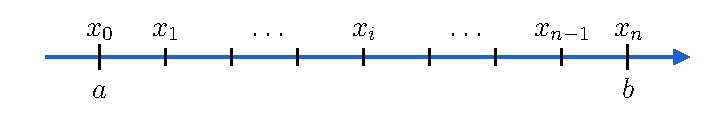
\includegraphics[width=\textwidth]{img/chapter2/finite_difference_grid.pdf}
    \end{center}
    \caption{An equidistant division of the domain $[a, b]$ in $n$ intervals.}
    \label{fig:c2_finite_difference_grid}
\end{figure}

The idea for these kinds of methods, is to discretize the integration domain $[a, b]$ into an equally spaced grid of points $a = x_0$, $x_1$, $\dots$, $x_i$, $\dots$, $x_{n-1}$, $x_{n} = b$, with $\Delta x$ the distance between two consecutive points. This discretization can be seen in figure \ref{fig:c2_finite_difference_grid}. The differential equation is now approximated by using finite difference expressions of the involved derivatives. For linear ordinary differential equations, this leads to a linear matrix-vector reformulation of the differential equation, which can be solved with classical linear algebra tools.

In this general technique constructing higher order methods is mostly as straightforward as using a more accurate finite difference approximation. But these methods become increasingly computationally expensive as more accuracy is required, or higher eigenvalues are requested.


\subsubsection{Finite difference scheme for the Sturm-Liouville equation}

Until around 1990 the best methods \cite{andrew_correction_1985,vandenberghe_accurate_1991} for approximating solutions to the Sturm-Liouville equation looked at the simpler form of the Schrödinger equation and employed a finite difference scheme. After the fact, they applied some corrections to improve the accuracy of higher eigenvalues. They experimented with which finite difference approximations to use. First they tried classical formulae, later on highly tuned exponential fitted formulae to better handle the oscillatory nature of the eigenfunctions were developed.

To illustrate this class of finite difference methods for Sturm-Liouville equations we will develop a simple version ourselves. This will allow us to appreciate the nuances of these methods more, and it will give us some ideas about the general advantages but also disadvantages of this technique. The Sturm-Liouville equations we will consider are given by
\begin{equation}\label{equ:c2_finite_difference_slp}
    -(p(x)y')' + q(x) y = \lambda w(w) y\text{.}
\end{equation}
Solutions consist of eigenvalues $\lambda$ and corresponding eigenfunctions $y(x)$ such that \eqref{equ:c2_finite_difference_slp} is satisfied on the domain $[a, b]$ with homogeneous Dirichlet boundary conditions $y(a) = y(b) = 0$.

As a first step we discretize the domain $[a, b]$ with $n+1$ equidistant points, as in figure \ref{fig:c2_finite_difference_grid}. The eigenfunctions $y(x)$ we are looking for, can now be approximated by values in each of the grid points $y(x_i) \approx y_i$. For translating this problem into a linear matrix-vector equation, we are missing one key component. We need a way to discretize the expression $(p(x) y')'$. For this, we apply the central second order finite difference formula for the first derivative twice, with half the step size. In more detail, the first derivative of a scalar function $f(x)$ can be approximated as:
$$
    f'(x) \approx \frac{f(x + h) - f(x - h)}{2h}\text{.}
$$

Applying this expression once to $(p(x) y')'$ in the point $x_i$, with step size $h = \frac{\Delta x}{2}$ gives:
$$
    (p(x) y')'(x_i) \approx \frac{1}{\Delta x}\left((p y')\left(x_{i+\frac{1}{2}}\right) - (p y')\left(x_{i-\frac{1}{2}}\right))\right)\text{.}
$$
Applying the finite difference formula a second time, with step size $\frac{\Delta x}{2}$ to approximate $y'(x)$ yields:
$$
    (p(x) y')'(x_i) \approx \frac{1}{\Delta x^2}\left(p_{i+\frac{1}{2}} y_{i+1} - \left(p_{i-\frac{1}{2}} + p_{i+\frac{1}{2}}\right) y_i + p_{i-\frac{1}{2}} y_{i-1}\right)
$$
To ease notation we have substituted $y(x_i)$ with its approximation $y_i$, and have denoted $\frac{x_i + x_{i+1}}{2}$ as $x_{i+\frac{1}{2}}$, and $p(x_i)$ as $p_i$. Also, note that if $p(x) = 1$ this formula simplifies to the classical, well-known, central second order approximation of the second derivative.

If we apply this finite difference approximation to \eqref{equ:c2_finite_difference_slp} in each point $x_i$. We get the linear generalized eigenvalue problem:
$$
    -\frac{1}{\Delta x^2}\left(p_{i+\frac{1}{2}} y_{i+1} - \left(p_{i-\frac{1}{2}} + p_{i+\frac{1}{2}}\right) y_i + p_{i-\frac{1}{2}} y_{i-1}\right) + q(x_i) y_i = \lambda w(x_i) y_i \text{.}
$$

To emphasize that this is a linear algebra problem we can rewrite this in matrix notation:
\begin{equation}\label{equ:c2_finite_difference_matrix_problem}
    \left(-\vb{D} + \diag(\vb{q})\right)\vb{y} = \lambda \diag(\vb{w}) \vb{y}\text{.}
\end{equation}

The $(n-1)$-dimensional vector $\vb{y} = \transpose{\begin{pmatrix}y_1 & y_2 & \dots & y_{n-1}\end{pmatrix}}$ is the unknown approximation of the eigenfunction. The $(n-1)$-dimensional vectors $\vb{q} = \transpose{\begin{pmatrix}q(x_1) & q(x_2) & \dots & q(x_{n-1})\end{pmatrix}}$  and $\vb{w} = \transpose{\begin{pmatrix}w(x_1) & w(x_2) & \dots & w(x_{n-1})\end{pmatrix}}$ are the values of the coefficient functions $q$ and $w$. And lastly, the matrix $\vb{D}$ is the tridiagonal matrix given by:
$$
    \vb{D} = \frac{1}{\Delta x^2}\begin{pmatrix}
        -p_{\frac{1}{2}} -p_{\frac{3}{2}} & p_{\frac{3}{2}}                   &                                   &                     &                                            \\
        p_{\frac{3}{2}}                   & -p_{\frac{3}{2}} -p_{\frac{5}{2}} & p_{\frac{5}{2}}                   &                     &                                            \\
                                          & p_{\frac{5}{2}}                   & -p_{\frac{5}{2}} -p_{\frac{7}{2}} & p_{\frac{7}{2}}     &                                            \\
                                          &                                   &                                   & \ddots              &                                            \\
                                          &                                   &                                   & p_{n - \frac{3}{2}} & -p_{n - \frac{3}{2}} - p_{n - \frac{1}{2}} \\
    \end{pmatrix}{}\text{.}
$$

To find the eigenvalues of \eqref{equ:c2_finite_difference_matrix_problem} one can notice that if $w(x_i)$ is never $0$ for $0 < i < n$ then $\diag(\vb{w})$ is invertible and the problem becomes a simple tridiagonal eigenvalue problem. This can then be solved with any of our favorite tridiagonal eigenvalue solver. If $w$ happens to be constant, this becomes a symmetric tridiagonal matrix, for which LAPACK \cite{lapack}, for example, contains the specialized routines: \texttt{?stev} and relatives.

\begin{figure}
    \begin{center}
        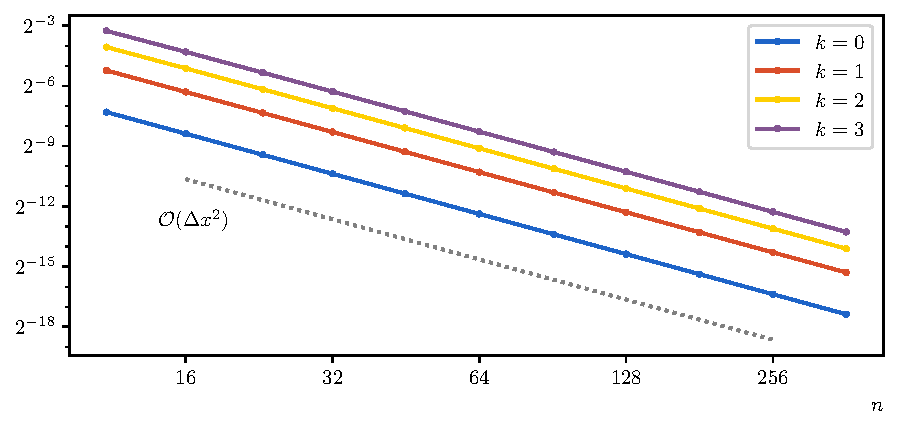
\includegraphics[width=\textwidth]{img/chapter2/finite_difference_h_error.pdf}
    \end{center}
    \caption{Relative error of approximated eigenvalues of problem \eqref{equ:c2_fd_test_problem} in function of the grid size $n$ on the domain.}
    \label{fig:c2_fd_h_error}
\end{figure}

\begin{figure}
    \begin{center}
        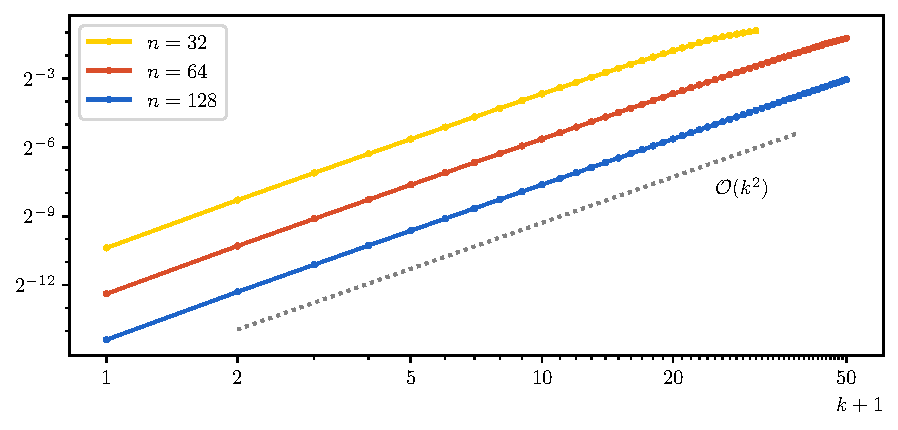
\includegraphics[width=\textwidth]{img/chapter2/finite_difference_k_error.pdf}
    \end{center}
    \caption{Relative error of approximated eigenvalues of problem \eqref{equ:c2_fd_test_problem} in function of the eigenvalue index $k$.}
    \label{fig:c2_fd_k_error}
\end{figure}

As a numerical experiment of this method we will take a look at the following Sturm-Liouville equation:
\begin{equation}\label{equ:c2_fd_test_problem}
    -\left((1+x)^2 y \right)' + (x^2 - 2) y = \lambda e^x y
\end{equation}
on the domain $[0, 1]$ with homogeneous Dirichlet boundary conditions. Figure \ref{fig:c2_fd_h_error} shows the relative errors of the 4 lowest eigenvalues in function of the chosen grid size $n$. As $n$ increases, the error decreases, as desired. Notice that as the constructed method is based upon second order finite difference formulae, we expect to see the decrease of error be of second order too, as indicated in the figure with the dotted line. This constructed method is of relatively low order, so to compute very accurate estimations, a dense grid is needed. In the literature one can find many methods base upon finite difference approximations, many of which use (much) higher order formulae. These better methods can reach high accuracy with relatively little computational work, for the first few eigenvalues.

As earlier hinted, methods based upon finite differences struggle with the computation of higher eigenvalues. Figure \ref{fig:c2_fd_k_error} illustrates this. Here, the relative error of the first 50 eigenvalues is plotted, for different values of $n$. Note that in the case of $n = 32$, only $32$ eigenvalues can be computed. On this figure, the line corresponding to $\mathcal{O}(k^2)$ is drawn. Together with the $\mathcal{O}(\Delta x^2)$ from earlier, one expects the relative error of the $k^\text{th}$ eigenvalue to be
$$
    \mathcal{O}(\Delta x^2 k^2)
$$
for this method applied to problem \eqref{equ:c2_fd_test_problem}. This teaches us for this method in particular, but it is also applicable to most methods of this type, that the larger the eigenvalue, the more difficult it is to compute accurately. In the literature one can find some techniques to mitigate this effect by applying some corrections after the fact. In \cite{andrew_correction_1985} such a correction is analyzed when applied to Numerov's method. Here, the authors are able to bring the error down from $\mathcal{O}(k^6 h^4)$ to $\mathcal{O}(k^3 h^4)$. This is remarkably better. But even with this correction technique, computing large eigenvalues is still computationally difficult.

\subsection{CP-methods}

The drawbacks of the methods based upon finite differences are already known for a long time. One of the first\footnote{In \cite{ledoux_solving_2010} a brief historical overview is given of the application of CP-methods to Sturm-Liouville problems. In this thesis we will take the time to take a closer look at the earlier methods. They will provide us a more intuitive understanding of the algorithms, in preparation of our own advancements within employing these ideas.} works that tries to not only mitigate these troubles but rather fully fix them, was \cite{canosa_new_1970} in 1970. There, Canosa and De Oliveira present a new method to approximate solutions to the one dimensional time-independent Schrödinger equation. Here, the foundations are build to what would later be called constant perturbation methods (CPM or CP-methods). To intuitively appreciate these CP-methods it is valuable to study the method from \cite{canosa_new_1970}.

For this, we will only consider the Schrödinger equation
\begin{equation}\label{equ:c2_cpm_schrodinger}
    - y'' + V(x) y = \lambda y
\end{equation}
on the domain $[a, b]$ with homogeneous Robin boundary conditions $\alpha_a y(a) + \beta_a y(a) = 0$ and $\alpha_b y(b) + \beta_b y(b) = 0$. But do note, that using Liouville's transformation Sturm-Liouville problems can be transformed into Schrödinger problems.

\subsubsection{Piecewise constant approximation of the potential}

\begin{figure}
    \begin{center}
        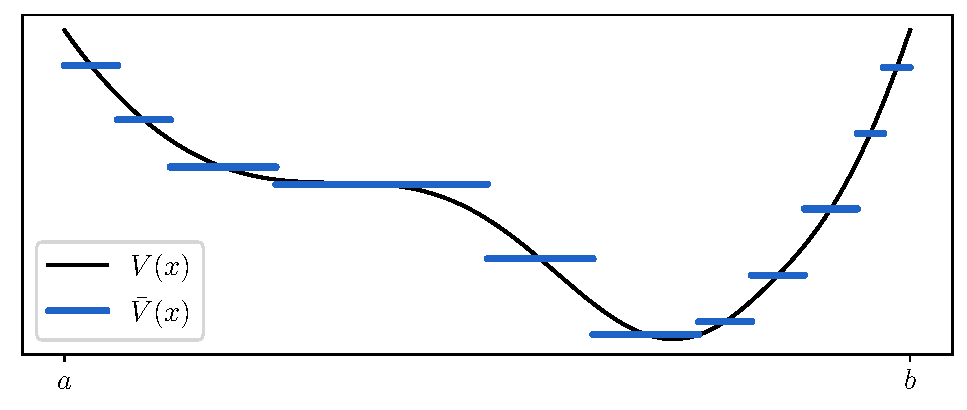
\includegraphics[width=\textwidth]{img/chapter2/cpm_constant_approx.pdf}
        \caption{A potential function $V(x)$ is approximated as the piecewise constant function $\bar{V}(x)$ along the domain $[a, b]$.}
        \label{fig:c2_cpm_constant_approx}
    \end{center}
\end{figure}

As a very first step, \cite{canosa_new_1970} simplifies the potential $V(x)$ as a piecewise constant approximation $\bar{V}(x)$. This approximation is visualized in figure \ref{fig:c2_cpm_constant_approx}. Notice that no restrictions are placed upon the size of the pieces. Upon choosing $\bar{V}(x)$, one should keep in mind that the better the piecewise approximation is, the better the resulting eigenvalues will be. And, the computational runtime depends linearly on the number of pieces.

The next step is to fix the value for $\lambda$ for now. Then, for each of the pieces of $\bar{V}$ the analytical solutions is computed of the problem
$$
    y'' = (V_i - \lambda) y\text{.}
$$
Here, $V_i$ is the value of $\bar{V}$ on the $i^\text{th}$ piece $[x_i, x_{i+1}]$. These analytical solutions $\psi_i(x)$ have the following structure.
$$
    \psi_i(x) = \begin{cases}
        A_i + B_i x                                                         & \text{ if $V_i = \lambda$} \\
        A_i \cos(x\sqrt{\lambda - V_i}) + B_i \sin(x\sqrt{\lambda - V_i})   & \text{ if $V_i < \lambda$} \\
        A_i \cosh(x\sqrt{V_i - \lambda}) + B_i \sinh(x\sqrt{V_i - \lambda}) & \text{ if $V_i > \lambda$}
    \end{cases}
$$

To determine the appropriate values for $A_i$ and $B_i$ continuity conditions between pieces are applied:
$$
    \psi_{i-1}(x_i) = \psi_{i}(x_i) \text{ and } \psi_{i-1}'(x_i) = \psi_{i}'(x_i) \text{.}
$$
If $n$ pieces are used, this system of equations has $2n$ variables and $2(n-1)$ equations. Together with the two equations from the boundary conditions, this yields a fully determined linear system. Now, we have translated the problem of finding eigenvalues of the Schrödinger equation \eqref{equ:c2_cpm_schrodinger} to finding values for $\lambda$ such that this system of equations has non-zero solutions. Only these solutions correspond to a non-zero eigenfunction.

Finding values for $\lambda$ for which the constructed system becomes singular is not as trivial as one may assume. In \cite{canosa_new_1970}, the authors have provided their own root finding algorithm based upon finding changes in the sign of the determinant. But this algorithm is not without issue. Eigenvalues may be arbitrarily close together, which makes it hard to ensure you have found all requested values. Choosing the appropriate step sizes when eigenvalues become increasingly sparse is a balance between efficiency and not missing any. Later on we will describe a way to reliably and efficiently determine all required eigenvalues.

One of the main benefits of this ``new method for the solution of the Schrödinger equation'' \cite{canosa_new_1970} is that its accuracy does not depend on the size of the requested eigenvalue. Because only analytical solutions of the piecewise approximated problem are considered, oscillations can be represented exactly. Even the most extreme oscillations are cleanly captured inside the $\sin$ en $\cos$ of $\psi_i$. The idea of using analytical solutions allowed the development of the CP-methods.

When studying this method one can make the observation when looking at figure \ref{fig:c2_cpm_constant_approx} that $\bar{V}(x)$ is a crude approximation of the function $V(x)$. The importance of this remark becomes even more apparent when one realizes that the accuracy of the method solely depends upon the accuracy of this approximation.

Nonetheless, the idea of Canosa and De Oliveira gained traction. In 1971 Ixaru \cite{ixaru_error_1972} has written a note about the error analysis of this new method. And in the same year Pruess \cite{pruess_estimating_1973} has studied this method thoroughly and provided numerical examples of linear piecewise approximations and quadratic piecewise approximations of the potential function. Here we will state the most important theorems, without proof. All details can be found in \cite{pruess_estimating_1973}.

\begin{theorem}[Pruess 1973]\label{the:c2_pruess_1973_1}
    Let $\lambda_k$ be the $k^\text{th}$ eigenvalue of the Schrödinger equation
    $$
        -y'' + V(x) y = \lambda y
    $$
    on the domain $[a, b]$ with homogeneous Robin boundary conditions. And let $\tilde{\lambda}_k$ be the $k^\text{th}$ eigenvalue of the approximate Schrödinger equation with potential $\bar{V}(x)$ on the same domain, with identical boundary conditions. Here $\bar{V}(x)$ is a piecewise $m^\text{th}$ degree polynomial approximation, let $h$ be the width of the largest piece in this approximation. For $h$ sufficiently small, we have as $h \to 0$,
    $$
        |\lambda_k - \tilde{\lambda}_k| = \mathcal{O}(h^{2m + 2}) \text{ for each $k$.}
    $$
\end{theorem}

This theorem provides justification for the idea of Canosa and De Oliveira. Even though a constant approximation ($m = 0$) may be crude, it still is a second order method. Furthermore, the theorem suggest that expanding this method up to higher degree piecewise polynomial approximations may be worthwhile.

In \cite{pruess_estimating_1973}, the author also studies what happens to the error on the eigenvalues if $k$ is increased. In \cite{canosa_new_1970} it was assumed that this error does not get worse as $k$ increases.

\begin{theorem}[Pruess 1973]\label{the:c2_pruess_1973_2}
    Following the notation from theorem \ref{the:c2_pruess_1973_1}, assume $\bar{V}(x)$ to be a least squares $m^\text{th}$ degree piecewise polynomial approximation of $V(x)$. This means, on each piece $[x_i, x_{i+1}]$, that $\bar{V}$ is the $m^\text{th}$ degree polynomial such the following is minimal
    $$
        \int_{x_i}^{x_{i+1}} \left(V(x) - \bar{V}(x)\right)^2 \dd x \text{.}
    $$

    Under this assumption, if $k \to \infty$, it holds for the relative error that
    $$
        \frac{\lambda_k - \tilde{\lambda}_k}{\lambda_k} = \mathcal{O}(k^{-4})\text{.}
    $$
\end{theorem}

This last theorem does not only say that the error does not become larger if $k$ increases, but the relative error even decreases rapidly when $k \to \infty$. Theorem \ref{the:c2_pruess_1973_2} highlights the main advantage this technique has in comparison to other state-of-the-art methods. Where many other methods become less and less accurate for large eigenvalues, this method becomes even more accurate.

\begin{figure}
    \begin{center}
        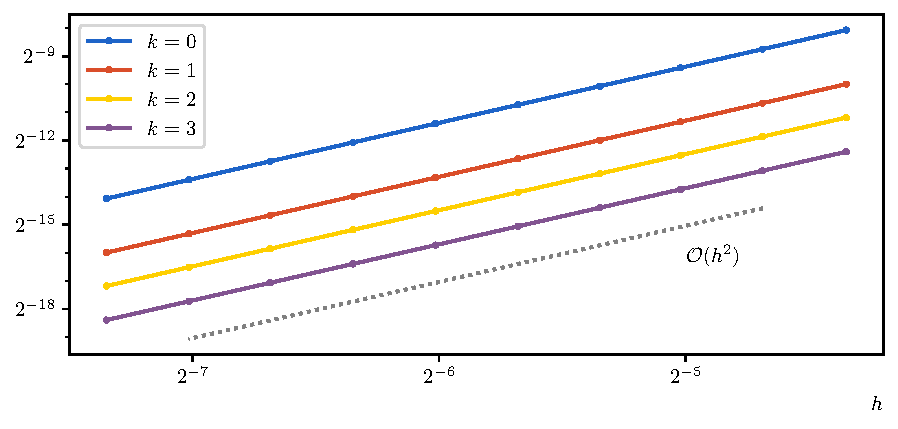
\includegraphics[width=\textwidth]{img/chapter2/pruess_h_error.pdf}
    \end{center}
    \caption{Relative error of the found eigenvalues of problem \eqref{equ:c2_pruess_test_problem} by using the method of constant piecewise approximation of the potential, with equal pieces. The graphs are in function of the size of the pieces. The most accurate calculation used $512$ pieces, the least accurate $64$.}
    \label{fig:c2_pruess_h_error}
\end{figure}

\begin{figure}
    \begin{center}
        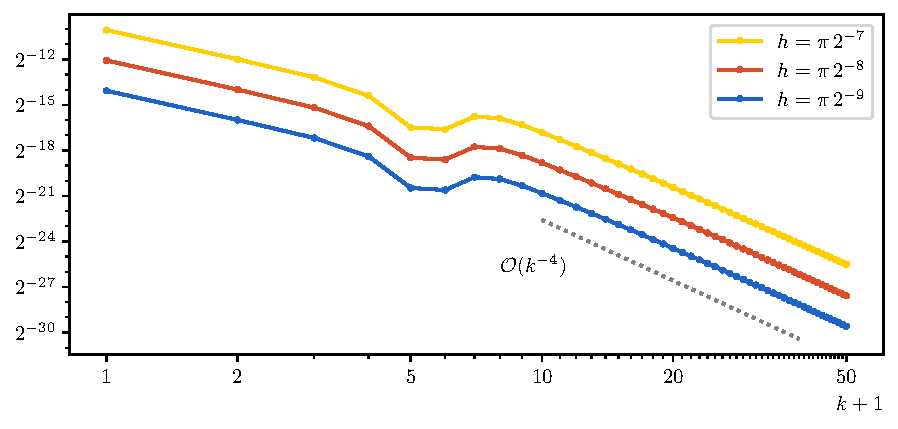
\includegraphics[width=\textwidth]{img/chapter2/pruess_k_error.pdf}
    \end{center}
    \caption{Relative error of the found eigenvalues of problem \eqref{equ:c2_pruess_test_problem} by using the method of constant piecewise approximation of the potential, with equal pieces. The graphs are in function of the index of the eigenvalue. The yellow line used $128$ pieces, the blue line $512$.}
    \label{fig:c2_pruess_k_error}
\end{figure}

As a numerical experiment we have applied the method with constant piecewise approximations ($m=0$) to the Mathieu problem
\begin{equation}\label{equ:c2_pruess_test_problem}
    -y'' + 100 \cos(x)^2 y = \lambda y
\end{equation}
on the domain $[0, \pi]$ with homogeneous Dirichlet boundary conditions. In figure \ref{fig:c2_pruess_h_error} the relative error of the application of the method is illustrated. We see that the error follows indeed the predicted line of $\mathcal{O}(h^2)$. In figure \ref{fig:c2_pruess_k_error} we see the dramatic increase in accuracy when $k$ becomes larger. The predicted order of $\mathcal{O}(k^{-4})$ seems to be reached once $k$ is sufficiently large.


But still some nuances have to be made. In \cite{pruess_estimating_1973} some numerical examples are given for constant ($m=0$), linear ($m=1$) and quadratic ($m=2$) approximations. But only for the constant approximations analytical solutions were used. For the higher order experiments, the true solution on a single piece is approximated by an at least fifteenth order Taylor series expansion. These Taylor series are only polynomial approximations of a possibly highly oscillatory function. Which, for much higher eigenvalues, gives problems.

\subsubsection{Constant perturbation methods}

In the years since the first article from Canosa and De Oliveira \cite{canosa_new_1970}, the research into these kinds of methods has flourished. One of the first extensions considered not only piecewise constant approximations but also linear and quadratic approximations, as in \cite{pruess_estimating_1973}. For constant approximations, the exact solution is given by hyperbolic or trigonometric functions. For linear approximations, the Airy functions $\Ai(x)$ and $\Bi(x)$ are appropriate. As these are well-known special functions, software packages are available to evaluate them. But not unexpectedly, these packages are harder to find, and more difficult to use, than $\sin$, $\cos$ and hyperbolic variants. For quadratic, and higher order, approximations no closed form formula exists for the exact solutions.

To improve accuracy and computational efficiency, it is, when developing numerical methods, valuable to construct higher order methods. As we are limited to an order of $\mathcal{O}(h^2)$ for constant approximations, or $\mathcal{O}(h^4)$ when using linear approximations, some alternative improvements were required. In the book \cite{ixaru_numerical_1984}, Ixaru dedicated chapter 3 to the development of the constant perturbation methods. The main idea is to, not directly improve the approximation of $V(x)$. But, starting with a piecewise constant approximation $\bar{V}(x)$, adding correction terms to capture the difference between the reference solution for $\bar{V}(x)$ and the true solution for $V(x)$.

Before we deconstruct the constant perturbation methods, let us take the time to formalize which mathematical problem we are solving. For now, we will only look at the differential equation
\begin{equation}\label{equ:c2_cpm_corrected}
    y''(\delta) = (\Delta V(\delta) + \bar{V} - \lambda) y(\delta)
\end{equation}
as initial value problem starting from $0$. Denote the homogeneous Neumann solution as $u(\delta)$, as such, $u(0) = 1$ and $u'(0) = 0$. And, we will write the homogeneous Dirichlet solution as $v(\delta)$, thus $v(0) = 0$ and $v'(0)=1$. In \eqref{equ:c2_cpm_corrected}, $\bar{V}$ is a constant (not piecewise) approximation of $V(x)$ on the current piece $[x_i, x_{i+1}]$ and $\Delta V(\delta) := V(x_i + \delta) - \bar{V}$. Being able to solve the initial value problem is sufficient to also solve the boundary value eigenproblem. For solving the latter we can employ a shooting procedure to the former, see section \ref{sec:c2_shooting_prufer} for more details. The procedure we will develop here can then be applied to each of the pieces in the constant piecewise approximation of $V(x)$.

Following \cite{ixaru_numerical_1984,ixaru_cp_2000}, let us denote a solution of \eqref{equ:c2_cpm_corrected} generally as $p(\delta)$, this thus represents either $u(\delta)$ or $v(\delta)$. Now we write the solution $p(\delta)$ as a perturbation series:
$$
    p(\delta) = p_0(\delta) + p_1(\delta) + p_2(\delta) + \dots
$$
In this expression the first order term $p_0$ is the solution of the reference equation
\begin{equation}\label{equ:c2_p0_reference}
    p_0''(\delta) = (\bar{V} - \lambda) p_0(\delta)
\end{equation}
with appropriate initial values. That is, $u_0(0) = 1$ and $u_0'(0) = 0$ for $p = u$, if $p=v$ the initial values are $v_0(0)=0$ and $v_0'(0) = 1$. The perturbation corrections can now be recursively defined as the solution of
\begin{equation}\label{equ:c2_pq_definition}
    p_q''(\delta) = (\bar{V} - \lambda) p_q(\delta) + \Delta V(\delta) p_{q-1}
\end{equation}
with initial conditions $p_q(0) = p_q'(0) = 0$. Notice that this definition implies that $p$ indeed solves \eqref{equ:c2_cpm_corrected} with the appropriate initial values:
\begin{align*}
    p'' & = (\bar{V} - \lambda)p_0 + \sum_{q=1}^\infty\left((\bar{V} - \lambda)p_q + \Delta V(\delta) p_{q-1}\right) \\
        & = (\bar{V} - \lambda)\sum_{q=0}^\infty p_q + \Delta V(\delta) \sum_{q=0}^\infty p_q                        \\
        & = (\Delta V(\delta) + \bar{V} - \lambda)p\text{.}
\end{align*}

To symbolically compute the expression of $p_q$ Ixaru has introduced some auxiliary functions\footnote{What we will call $\eta_{-1}$, Ixaru has named $\xi$. The notation of the recursive definition becomes a little easier when the $\eta_m$ and $\xi$ names are unified.}, based upon the exact solution of the constant perturbation method.

\begin{definition}[Ixaru 1984]\label{def:c2_eta_functions}
    The family of $\eta$-functions $\eta_m : \RR \to \RR$ for $m \in \{-1, 0, 1, \dots\}$ is defined recursively as:
    \begin{align*}
        \eta_{-1}(Z) & = \cosh(\sqrt{Z})                                        \\
        \eta_{0}(Z)  & = \frac{\sinh(\sqrt{Z})}{\sqrt{Z}}                       \\
        \eta_{m}(Z)  & = \frac{\eta_{m-2}(Z) - (2m-1) \eta_{m-1}(Z)}{Z}\text{.}
    \end{align*}
    When $Z < 0$ the definitions of $\eta_{-1}$ and $\eta_{0}$ should be read as calculations in $\CC$. But, notice that the resulting values will always be real. Furthermore, if $Z = 0$, one should take the limit of $\eta_m$ to zero, this yields\footnote{In this expression $n!!$ is the double factorial: $n!! := n\cdot (n-2) \cdot (n - 4) \cdot ...$, with only strictly positive integers as factors. For our purposes we define $0!! = (-1)!! = 1$.} $\eta_m(0) = \frac{1}{(2m+1)!!}$.
\end{definition}

When implementing these formulas, it is more efficient to keep all calculations in $\RR$. For $Z < 0$ we implement $\eta_{-1}(Z) = \cos(\sqrt{-Z})$ and $\eta_{-1}(Z) = \sin(\sqrt{-Z})/\sqrt{-Z}$.

Another interesting property of these $\eta$-functions are its series expansions:\begin{align*}
    \eta_{-1}(Z) & = \sum_{q=0}^{\infty} \frac{Z^q}{(2q + 1)!}                                                      \\
    \eta_{m}(Z)  & = 2^m \sum_{q=0}^{\infty} \frac{(q+m)! Z^q}{q!(2q + 2m + 1)!} \qquad \text{if } m \geq 0\text{.}
\end{align*}
When $|Z|$ is small, the recursion from the definition becomes numerically unstable. It is more accurate to use this series expansion on $\eta_m$ and $\eta_{m+1}$, for $m$ sufficiently large, and work our way back to $m=0$ and $m=-1$ with the inverted recursion
$$
    \eta_{m-1}(Z) = Z \eta_{m+1}(Z) + (2 m + 1) \eta_{m}(Z)
    \text{.}
$$

Other interesting properties of these special functions are already studied. Here we provide some results, without proofs.
\begin{theorem}[Ixaru 1984]\label{the:c2_eta_functions}
    For the family of functions defined in definition \ref{def:c2_eta_functions}, the following properties hold for $m \in \{-1, 0, 1, 2, \dots\}$ and $Z \in \RR$.
    \begin{itemize}
        \item Asymptotic behavior for $|Z| \to \infty$:
              $$\eta_m(Z) \approx  \begin{dcases}
                      \frac{\eta_{-1}(Z)}{Z^{(m+1)/2}} & \text{if $m$ is odd}  \\
                      \frac{\eta_{0}(Z)}{Z^{m/2}}      & \text{if $m$ is even}
                  \end{dcases}$$
        \item Differentiation with respect to $Z$:
              $$
                  \eta'_{m}(Z) = \frac{1}{2}\eta_{m+1}(Z)
              $$
        \item Differentiation with respect to $\delta$ if $Z = F\delta^2$:
              \begin{align*}
                  \pdv[]{\eta_{-1}(Z)}{\delta}             & = \frac{Z}{\delta} \eta_0(Z)                           \\
                  \pdv[]{\delta^{2m+1}\eta_{m}(Z)}{\delta} & = \delta^{2m} \eta_{m-1}(Z) \qquad \text{if } m \geq 0 \\
              \end{align*}
    \end{itemize}
\end{theorem}

With the theory about the family of $\eta$-functions in hand, we are able to solve equations \eqref{equ:c2_p0_reference} and \eqref{equ:c2_pq_definition} symbolically. The following theorem from \cite{ixaru_numerical_1984} captures these symbolic calculations for $p_q(\delta)$. As these formulae have been instrumental to our work (especially for section \ref{sec:c2_cp_in_delta}), we will provide a proof.

\begin{theorem}[Ixaru 1984]\label{the:c2_perturbation_terms}
    Let $p(\delta)$ be a general solution of
    $$
        p''(\delta) = \left(\Delta V(\delta) + \bar{V} - \lambda\right)p(\delta)
    $$
    over the interval $[0, h]$. In this expression $V = \bar{V} + \Delta V(\delta)$ is a given potential function, with $\bar{V}$ a constant approximation and $\Delta V(\delta)$ the residual term. The value $\lambda$ is fixed. We denote the solution with initial conditions $u(0) = 1$ and $u'(0)=0$ as $u(\delta) = p(\delta)$, and the solution with initial conditions $v(0) = 0$ and $v'(0) = 1$ will be denoted with $v(\delta) = p(\delta)$. For ease of notation we will write $Z(\delta) = \left(\bar{V} - \lambda\right)\delta^2$. Let $p(\delta) = p_0(\delta) + p_1(\delta) + p_2(\delta) + \dots$ with:
    \begin{align*}
        p_0''(\delta) & = (\bar{V} - \lambda) p_0(\delta)                                                             \\
        p_q''(\delta) & = (\bar{V} - \lambda) p_q(\delta) + \Delta V(\delta) p_{q-1}(\delta) \quad\text{for $q > 0$.}
    \end{align*}
    The function $p_0$ inherits the initial conditions of $p$. If $q > 0$, $p_q$ has as initial conditions $p_q(0) = p_q'(0) = 0$.


    If $\Delta V(\delta)$ is a polynomial in $\delta$ then each term \(p_q\) is given by:
    \begin{align}
        p_q(\delta)  & = \sum_{i=-1}^\infty \delta^{2i+1} C^{(q)}_i(\delta) \eta_{i}(Z(\delta))  \label{equ:c2_cp_coeff_pq_formula}                                             &
        \intertext{with derivative:}
        p_q'(\delta) & = \frac{C_{-1}^{(q)}(\delta)}{\delta^2}\left(\eta_{-1}(Z(\delta))+Z(\delta)\eta_{0}(Z(\delta))\right)            \label{equ:c2_cp_coeff_pq_diff_formula}   \\\nonumber
                     & \qquad + \sum_{i=-1}^\infty \left(C_{i}^{(q)\prime}(\delta) + \delta C_{i+1}^{(q)}(\delta)\right) \delta^{2i + 1}\eta_{i}(Z(\delta)) \text{.}
    \end{align}
    The functions $ C^{(q)}_i (\delta) $ are polynomials and satisfy the following recursive relation: \begin{align*}
        C_i^{(q)}(\delta)    & = \frac{\delta^{-i}}{2} \int_0^\delta \varepsilon^{i-1} \left(
        C_{i-1}^{(q-1)}(\varepsilon) \Delta V(\varepsilon) - C_{i-1}^{(q)\prime\prime}(\varepsilon)
        \right)\dd\varepsilon                                                                 \\
        C_{i}^{(0)}(\delta)  & = \begin{cases}
            \delta & \text{if $p = u$ and $i = -1$} \\
            1      & \text{if $p = v$ and $i = 0$}  \\
            0      & \text{otherwise}
        \end{cases}                                   \\
        C_{-1}^{(q)}(\delta) & = 0 \quad \text{if $q > 0$}\,.                                 \\
    \end{align*}
\end{theorem}
\begin{proof}
As these formulae are recursively defined, a proof by induction is most natural. For $q=0$ the exact solutions can be calculated. If $\bar{V} \geq \lambda$, then $u_0(\delta) = \cosh(\sqrt{Z(\delta)})$ and $v_0(\delta) = \sinh(\sqrt{Z(\delta)})/\sqrt{\bar{V} - \lambda}$. If $\bar{V} < \lambda$ on the other hand, then $u_0(\delta) = \cosh(\sqrt{-Z(\delta)})$ and $v_0(\delta) = \sinh(\sqrt{-Z(\delta)})/\sqrt{\lambda - \bar{V}}$. By using the $\eta$-functions both these can be summarized as:
$$ u_0 = \eta_{-1}(Z(\delta)) \text{ and } v_0 = \delta\eta_{0}(Z(\delta))\text{.}$$
Substituting, for $q=0$, the values of $C^{(0)}_i$ into \eqref{equ:c2_cp_coeff_pq_formula} yields exactly the same expressions. This proves the induction basis.

Assume, as induction hypothesis, that the theorem holds for any value for $q$ less than $Q$. First we prove that for each $i$, $C_i^{(Q)}$ is a polynomial. For this we apply induction with respect to $i$. For $i = -1$, the $C^{(Q)}_{-1} =0$ is a polynomial. Because $\Delta V(\delta)$ is assumed to be polynomial, we notice that for any other $i$
$$
    C_{i-1}^{(Q-1)}(\varepsilon) \Delta V(\varepsilon) - C_{i-1}^{(Q)\prime\prime}(\varepsilon)
$$
is a polynomial, as a consequence of the induction hypothesis in $Q$, and the induction hypothesis in $i$. This implies that the integrand in the definition of $C_i^{(Q)}(\delta)$ is polynomial no terms of degree less than $i-1$. This means that the integral in that definition will be divisible by $\delta^i$. Which proves that all $C_{i}^{(Q)}$ are polynomials.

Next we proof that $p_Q(\delta)$ is a solution of
$$
    p_Q''(\delta)  = (\bar{V} - \lambda) p_Q(\delta) + \Delta V(\delta) p_{Q-1}(\delta)
$$
with initial conditions $p_Q(0) = p_Q'(0) = 0$. That $p_Q(0) = 0$ can be seen in \eqref{equ:c2_cp_coeff_pq_formula}, using the facts that $C^{(Q)}_{-1} = 0$ for $Q > 0$ and that $C_i^{(Q)}$ are polynomials. Using the properties from theorem \ref{the:c2_eta_functions}, we can compute $p_Q'(\delta)$ to be as in \eqref{equ:c2_cp_coeff_pq_diff_formula}. That this expression is zero for $\delta = 0$ is less apparent. First, notice that most terms are zero because $C_i^{(Q)}$ are polynomials and $C^{(Q)}_{-1} = 0$ for $Q > 0$. The only term for which this is not clear is with $i = -1$: $C_0^{(Q)}(0)\eta_{0}(Z(0))$. For this term, we remark that the polynomial $C^{(q)}_{-1}(\delta)$ never contains a constant term, for most values of $q$ it is zero, and for $q=0$ it can only be zero or $\delta$. This means, by the recursive construction, that $C_{i}^{(q)}(\delta)$ also does not contain a constant term. Which means $C_{i}^{(q)}(0) = 0$, and thus $p_Q'(0) = 0$, for $Q > 0$. The last thing, we still have to proof, is that this $p_Q$ indeed solves its defining equation.

For this, we compute $p_Q''$. For the sake of brevity, we will omit the argument $\delta$ from most functions, and remember that all derivatives are with respect to $\delta$. But first, we know, from the definition of $C_i^q$ that
$$
    C_i^{(q)\prime} = -i \delta^{-1} C_i^{(q)} + \frac{\delta^{-1}}{2}\left(C^{(q-1)}_{i-1}\Delta V - C^{(q)\prime\prime}_{i-1}\right)\text{,}
$$
but also that
\begin{align*}
    {\dv[]{\delta^{2i+1}\eta_i(Z)}{\delta}}               & = \delta^{2i} \eta_{i-1}                                         \\
    \text{ and } {\dv[2]{\delta^{2i+1}\eta_i(Z)}{\delta}} & = \delta^{2i-1}\left(2i\eta_{i-1}(Z) + Z\eta_i(Z)\right)\text{.}
\end{align*}

\begingroup
\allowdisplaybreaks
These expressions, together with $C_{-1}^{(Q)} = 0$, now can be used to simplify $p_Q''$:
\begin{align*}
    p_Q   & = \sum_{i=0}^{+\infty} C_{i}^{(Q)} \delta^{2i + 1} \eta_{i}(Z)                                                                            \\
    p_Q'' & = \sum_{i=0}^{+\infty} C_i^{(Q)}\delta^{2i-1}\left(2i\eta_{i-1}(Z) + Z\eta_i(Z)\right)                                                    \\
          & + \sum_{i=-1}^{+\infty} 2C_{i+1}^{(Q)\prime}\delta^{2i+2}\eta_{i}(Z) + \sum_{i=0}^{+\infty} C_i^{(Q)\prime\prime}\delta^{2i+1}\eta_{i}(Z) \\
          & = \sum_{i=0}^{+\infty} C_i^{(Q)}\delta^{2i-1}\left(2i\eta_{i-1}(Z) + Z\eta_i(Z)\right)                                                    \\
          & + \sum_{i=-1}^{+\infty} -2(i+1)C_{i+1}^{(Q)}\delta^{2i+1}\eta_{i}(Z) + p_{Q-1} \Delta V                                                   \\
          & = \frac{Z}{\delta^2}p_Q + p_{Q-1} \Delta V \text{.}
\end{align*}
\endgroup
Due to the definition of $Z = \delta^2(\bar{V} - \lambda)$, this expresses exactly that $p_Q$ is a solution to $p_Q'' = (\bar{V} - \lambda)p_Q + \delta V p_{Q-1}$. Which, in turn, proves the induction step.
\end{proof}

At first glance, it may not be clear why theorem \ref{the:c2_perturbation_terms} is that important. Still, these rather tedious computations and relatively complicated recursive relation allows us to analytically construct formulae of any order. To calculate such a formula choose values $N$ and $Q$ and compute the values of $C_{i}^{(q)}$ for $q \leq Q$ and $i \leq N$. If $\Delta V$ is assumed to be a polynomial in $\delta$, then $C_{i}^{(q)}$ will be as well. The solution $p(\delta)$ will now take the following form:
$$
    p(\delta) = \sum_{q=0}^{Q} p_q(\delta) \text{ with } p_q(\delta) = \sum_{i=-1}^{N} C_{i}^{(q)}(\delta) \delta^{2i+1} \eta_i(Z) \text{.}
$$


\todo{(1)}

However, these formulae only can be calculated in case $V(x)$ is a polynomial. For this, the very first step in the CP-algorithm is to approximate $V(x)$ on each sector by a polynomial $V^{N}(x)$ of sufficient high degree $N$. One possible polynomial representation is by expressing it in terms of the orthogonal family of shifted Legendre polynomials $\widetilde{P}_n(\frac{\delta}{h})$. This family of polynomials satisfy\footnote{Here $\delta_{mn}$ is the Kronecker $\delta$, defined as $\delta_{mn} = 1$ if $m=n$ else $\delta{mn} = 0$.}
$$
\int_0^1 \widetilde{P}_m(x) \widetilde{P}_n(x) \dd x = \frac{\delta_{mn}}{2n + 1} \quad\text{ for $m \neq n$,}
$$
and are increasing in degree, together with $\widetilde{P}_n(x) = 1$ for any $n$. As a reference we provide the first four.
\begin{align*}
    \widetilde{P}_0(x) =& 1 & \widetilde{P}_2(x) =&6x^2 - 6x + 1 \\
    \widetilde{P}_1(x) =& 2x - 1 & \widetilde{P}_3(x) =&20 x^3 - 30 x^2 +12 x - 1
\end{align*}

Applying a least squares approximation of $V(\delta)$ with $N + 1$ shifted Legendre polynomials yields
$$
V(\delta) \approx \sum_{n=0}^N V_n h^n \widetilde{P}_n(\frac{\delta}{h})
$$
where
\begin{equation}\label{equ:c2_legendre_V}
    V_n= \frac{2 n + 1}{h^{n+1}} \int_0^h V(\delta) \widetilde{P}_n(\frac{\delta}{h}) d \delta, \quad \text{ with $n \in \{0, 1,\dots, N\}$.}
\end{equation}
To implement this, the numerical value of the integral can be computed with Gauss quadrature rules of sufficiently high degree.

Let us denote the constant perturbation method with given choices for the degree $N$ and the number of correction terms $Q$ as CPM$[N,Q]$, we have the following result \cite{ixaru_cp_1998}

\begin{theorem}\label{the:c2_h_error_estimate}
    If $\text{CPM}[N,Q]$ is applied to propagate the solution on an equidistant partition with mesh size $h$ then
    \begin{itemize}
        \item for small values of $E$ (i.e.\ if $Z$ remains sufficiently small), the error in the mesh points is bounded by $C_N h^{2\,N+2}$ (for some constant $C_N$) provided that $Q \geq \left\lfloor \frac{2\,N}{3} \right\rfloor +1$ if $N \geq 1$ and $Q=0$ if $N=0$.
        \item if $E$ is such that $Z(h)\ll 0$ in all intervals, the error in the mesh points is bounded by $C^*_N h^{N}/ \sqrt{E}$  (for some constant $C^*_N$) provided that $Q \geq 1$  if $N \geq 1$ and $Q=0$ if $N=0$.
    \end{itemize}
\end{theorem}

Finally, one can simplify the expressions for the coefficients of the perturbation terms \(C^{(q)}_i\) by taking into account the orders $P_0$ (for small $Z$) and $P_{ass}$ (for negative $Z$ with $|Z| \gg 0$) that can be attained by the CPM$[N,Q]$ method. Some terms will contribute to the solution in higher orders of $h$, and so they do not need to be computed. This pruning then finally results in a method which was generically denoted as CPM$\{P_0, P_{ass}\}$. Later in theorem \ref{the:c2_delta_formulae}, we will prove that $P_{ass} = P_0$, thus we will denote our method as CPM$\{P_0\}$.

The original SLCPM12-code implemented the CPM$\{12,10\}$ algorithm. In the original Matslise package, a user could choose between several algorithms: CPM$\{12,10\}$, CPM$\{14,12\}$, CPM$\{16,14\}$, CPM$\{18,16\}$.
In Matslise 2.0 only CPM$\{18,16\}$ and CPM$\{16,14\}$ are implemented. The CPM$\{16,14\}$ method is used for propagation and the difference between the two methods is used for error estimation.

The CP methods have also been successfully applied to other types of problems, such as the so-called coupled channel Schrödinger-equations problem. Research in the past lead to the \fortran code \lilix \cite{ixaru_lilix_2002} and the \matlab code \matscs \cite{ledoux_numerical_2007}. These programs made it then possible to construct CP-based methods for solving the two-dimensional Schrödinger problem \cite{ixaru_new_2010} and the time-dependent one-dimensional Schrödinger problem \cite{ledoux_accurate_2014}.

In chapters \ref{cha:c3} and \ref{cha:c4} we will develop methods for the two-dimensional time-independent Schrödinger equation. These new methods are only possible, thanks to the accurate and efficient CP-methods for the one-dimensional problem.

\subsection{Shooting with Prüfer's transformation}\label{sec:c2_shooting_prufer}

\todo{Reread, rework, expand.}

In the CP algorithm, the boundary value problem is reformulated as two initial value problems, for a fixed
energy \(E\). The left boundary condition is converted into
\(\psi(x_\text{min}) = b_\text{min} \) and \(\psi'(x_\text{min}) = -a_\text{min}\). By
employing a multiple shooting method, solutions to the initial value
problem can be used to solve the eigenvalue problem as well.

At the start of the procedure, the domain \([x_\text{min}, x_\text{max}]\) is partitioned in \(K\) intervals. The $i^\text{th}$ interval can be written as $I_i = [x_{i-1}, x_{i}]$, with \(x_\text{min} = x_0, x_1, \dots, x_{K-1}, x_{K} = x_\text{max}\) the mesh points. Generically we can write such an interval as \(I = [X, X+h]\). The solution \(\psi\) can now be expressed as:
\begin{equation}
    \begin{pmatrix}\psi(X+\delta) \\ \psi'(X+\delta)\end{pmatrix}
    = \begin{pmatrix} u(\delta) & v(\delta) \\ u'(\delta) & v'(\delta) \end{pmatrix} \begin{pmatrix} \psi(X) \\ \psi'(X) \end{pmatrix} \,, \qquad %\text{ with } 
    0 \leq \delta \leq h \,. \label{equ:c2_cpm_propmatrix}
\end{equation}

The functions \(u(\delta)\) and \(v(\delta)\), called propagators,
satisfy the local Schrödinger equation (analogous for \(v(\delta)\)):
\begin{equation}
    - u''(\delta) + V(X+\delta) u(\delta) = E u(\delta) \label{sequ:c2_local_schrodinger}
\end{equation}
with the initial conditions \(u(0) = 1, u'(0)=0\) and
\(v(0) = 0, v'(0)=1\). The one-step propagation matrix
$$
    \vb{P}(\delta) = \begin{pmatrix} u(\delta) & v(\delta) \\ u'(\delta) & v'(\delta) \end{pmatrix}
$$
has determinant \(1\), so the inverse matrix can be easily constructed. Knowledge of this propagation matrix (and its inverse) is sufficient to advance the solution in both directions along the interval.


\section{Matslise 3.0}

\todo{Blind copy from published work}

Matslise 3.0 \cite{baeyens_fast_2020}.

In 2005 the first version of Matslise \cite{ledoux_matslise_2005}, A \textsc{matlab} package for solving Sturm-Liouville problems (SLP), was published. This program was a modern take on the successful
constant perturbation (CP) method based code SLCPM12 \cite{ixaru_slcpm12_1999}. It was the first implementation of CP
methods in the user friendly and then modern numerical computing environment \textsc{matlab}. Up to that
point most, if not all, of these programs for solving Sturm-Liouville problems (SLCPM12, SLEIGN, SLEDGE, \ldots) \cite{ixaru_slcpm12_1999,bailey_sleign2_2001,eastham_sledge_1996}
were written in Fortran.

Matslise provided a graphical user interface that made it easy for all
researchers to effectively solve the
Sturm--Liouville equation without any knowledge of a particular programming language. Before it's release, if one wanted to solve
a particular SLP, sufficient knowledge of Fortran was needed to implement the problem at hand.

In 2016 a new version, Matslise 2.0 \cite{ledoux_matslise_2016}, was
released. In this whole new version of Matslise generalized
CP methods for SLP were implemented. These new methods enabled one to solve the
SLP without explicitly transforming the equation to
the Liouville normal form. Avoiding this normalization also made it possible to solve new types of SLPs. As of this writing
Matslise 2.0 has been downloaded over a thousand times. This number proves the need of current research to solve the SLP
equation.

As the original Matslise modernized the implementation of SLCPM12, the need to remodernize this proven package has become apparent in our attempt to use, following the ideas of Ixaru in \cite{ixaru_new_2010}, the Matslise routines to solve the multidimensional Schrödinger equation.
This approach requires the fast and accurate computation of both the eigenvalues and the corresponding eigenfunctions of several 1D Schrödinger-problems.
The current Matslise 2.0 version however mainly focuses on the fast and accurate computation of eigenvalues and the graphical representation of the eigenfunction.
In Matslise 2.0 the eigenfunctions can be computed quite accurate and fast, but only in a limited set of points (depending on the partition of the integration interval).
The accurate computation of the eigenfunction over the whole integration interval however is time-consuming in the current implementation of Matslise 2.0.

In fact, this illustrates that Matslise 2.0 has not been built as a library of functions, but as a set of functions around a central GUI to solve SLP (and Schrödinger problems in particular).
Several other features illustrate this, such as the algorithm that is used to detect whether a given problem is singular and the automatic computation of the error estimates for the eigenvalues.
The algorithms are very useful for solving a particular SLP, but valuable computation time is lost if this detection or the error estimation is not needed.

These challenges were the main motivator for a more efficient
implementation of Matslise. We have considered different ways to
optimize Matslise, keeping in mind its main features, in particular its user friendliness,
one of the main reason for the development of the first version of Matslise.

\todo{rework}
This paper is organized as follows. In section 2, we first give an overview of the formulae behind the CP-algorithms. After this summary of previous research and developments, we present in section 3 an extension to these well-established formulae with new convergence results to enable more efficient computation of the eigenfunctions in arbitrary points in the domain.
In section 4 more details about the new implementation are given.
%Here some choices are motivated. These choices range from why certain features were omitted to the addition of some new features.
In section 5 numerical experiments are presented. %These examples illustrate that, in comparison to Matslise 2.O, the new implementation allows the faster computation of eigenvalues and eigenfunctions of Schrödinger problems with the same (or even higher) accuracy.
Finally, in section 6 we make some conclusions and look forward for future developments.

\subsection{The CP method for Schrödinger problems}\label{the-method}

CP methods have already been described extensively, see e.g.\ \cite{ixaru_numerical_1984,ixaru_cp_1998,ixaru_cp_2000,ledoux_cp_2004}. The main bricks for the CP method and related $\eta$-functions were laid in \cite{ixaru_numerical_1984}. We present a short overview for the Schrödinger equation in particular; for a more in depth explanation see the previously mentioned references.

The one dimensional time independent Schrödinger equation is of the form
\[
    -\psi''(x) + V(x)\psi = E\psi\text{.}
\] The function $V(x)$ is called the potential function.
This eigenvalue problem is mostly considered as a boundary value problem on
the interval \([x_\text{min}, x_\text{max}]\). We further assume that the boundary
conditions are separate, i.e.\ they can be expressed as
\[
    a_\text{min} \psi(x_\text{min}) + b_\text{min}\psi'(x_\text{min}) = 0
    \quad \mbox{and} \quad
    a_\text{max} \psi(x_\text{max}) + b_\text{max}\psi'(x_\text{max}) = 0\,
\]
with not both $a_\text{min}$ and $b_\text{min}$ zero (analogous for $a_\text{max}$ and $b_\text{max}$).



\subsection{New formulae for the computation of the eigenfunctions}\label{sec:c2_cp_in_delta}

In section \ref{the-method} we have provided an overview of the CP method to solve the one-dimensional Schrödinger equation. This method can be summarized in the following steps:
\begin{itemize}
    \item Split the domain $[a, b]$ in intervals $(a=x_0, x_1, x_2, \dots, x_k, \dots, x_n = b)$.
    \item For each interval $k$ write $X = x_{k-1}$ and $h = x_k - x_{k-1}$. \begin{itemize}
              \item Construct propagators $u(\delta)$ and $v(\delta)$ for $\delta \in [0, h]$, according to the formulae from Theorem \ref{the:c2_perturbation_terms}.
              \item A solution $\psi(x)$ can be calculated on the $k^\text{th}$ interval if $\psi(X)$ is known:
                    \begin{align*}
                        \psi(X+\delta)  & = u(\delta)\psi(X) + v(\delta)\psi'(X)   \\
                        \psi'(X+\delta) & = u'(\delta)\psi(X) + v'(\delta)\psi'(X)
                    \end{align*}
          \end{itemize}
    \item Employ multiple shooting to find solutions to the boundary value problem.
\end{itemize}

Up to now the perturbation terms for $u(\delta)$ and $v(\delta)$ given in Theorem \ref{the:c2_perturbation_terms} were only calculated and implemented with $\delta = h$. In that case, one not only obtains superconvergence as formulated in Theorem \ref{the:c2_h_error_estimate}, but there is also a major simplification in symbolic complexity. Nevertheless, for higher orders even these 'simplified' formulae are daunting to work with.
%So one can easily understand why theorem \ref{the:c2_h_error_estimate} only gives results in function of $h$.

For the efficient calculation of eigenfunctions in arbitrary points of the domain it would however be beneficial if the propagation terms were also implemented in function of $\delta$. To prove the corresponding mathematical results, we reformulate the expressions of the propagators in terms of $\theta=\delta/h$.

%To calculate these extended expressions we need first some mathematical background on how to construct them. Since Theorem \ref{the:c2_perturbation_terms} described the perturbation terms as a function of $\delta$. So not substituting this $\delta$ with $h$ gives expressions for the propagators in function of $\delta$.
%
%This extension is given in the appendix.
%
%Theorem \ref{the:c2_h_error_estimate} assumes that this substitution did happen, so it is no longer valid for our new extended formulae. We give a new theorem:
%To construct an error estimate in function of $h$ it is useful to substitute $\delta = h\theta$ in the expressions from theorem \ref{the:c2_perturbation_terms}.

Functions of $\theta$ will be denoted with a bar, like $\bar{C}(\theta) = C(\theta h)= C(\delta)$ and $\bar{u}_{q}(\theta) = {u}_{q}(\theta h) =u_{q}(\delta)$. Again $\bar{p}$ generically denotes  the functions $\bar{u}$ or $\bar{v}$. The CP-correction terms are now given by:
\begin{align}
     & \bar{p}_q(\theta) = \sum_{i=-1}^\infty h^{2i+1}\theta^{2i+1} \bar{C}^{(q)}_i(\theta) \eta_{i}(Z(h\theta))
    \intertext{with derivative:}
     & \begin{aligned}
        \bar{p}_q'(\theta) & = \sum_{i=-1}^\infty \left(\bar{C}_{i}^{(q)\prime}(\theta) + h^2 \theta \bar{C}_{i+1}^{(q)}(\theta)\right) h^{2i + 1} \theta^{2i + 1}\eta_{i}(Z) \\
                           & \quad \quad + \frac{\bar{C}_{-1}^{(q)}(\theta)}{\theta^2 h}\left(\eta_{-1}(Z)+Z\eta_{0}(Z)\right) \text{.}
    \end{aligned}
\end{align}
The functions \(\bar{C}^{(q)}_i\) satisfy the following recursive relation: \begin{align}
    \bar{C}_i^{(q)}(\theta)    & = \frac{\theta^{-i}}{2} \int_0^\theta \sigma^{i-1} \left(
    \bar{C}_{i-1}^{(q-1)}(\sigma) \Delta V(X+h\sigma) -  h^{-2} \bar{C}_{i-1}^{(q)\prime\prime}(\sigma)
    \right)\dd\sigma \nonumber                                                             \\
    \bar{C}_{i}^{(0)}(\theta)  & = \begin{cases}
        h\theta & \text{if $p = u$ and $i = -1$} \\
        1       & \text{if $p = v$ and $i = 0$}  \\
        0       & \text{otherwise}
    \end{cases}                              \\
    \bar{C}_{-1}^{(q)}(\theta) & = 0 \quad \text{if $q > 0$}\,.\nonumber
\end{align}


Denoting $\bar{\psi}(\theta) =\psi(X+\theta\,h)$, the propagation relation (\ref{equ:c2_cpm_propmatrix}) can be rewritten

\begin{equation}
    \begin{pmatrix}\bar{\psi}(\theta)\\ \bar{\psi}'(\theta)\end{pmatrix}
    = \begin{pmatrix} \bar{u}(\theta) & \bar{v}(\theta)/h \\ \bar{u}'(\theta) & \bar{v}'(\theta)/h \end{pmatrix} \begin{pmatrix} \bar{\psi}(0) \\ \bar{\psi}'(0) \end{pmatrix} \,, \qquad %\text{ with } 
    0 \leq \theta \leq 1 \,. \label{equ:c2_cpm_propmatrix2}
\end{equation}

\begin{theorem}[Baeyens and Van Daele 2020]\label{the:c2_delta_formulae}
    Assume, for $h$ sufficiently small, that an approximation of the propagation matrix % in $\theta = \frac{\delta}{h} \in [0, 1]$
    $$
        \begin{pmatrix}
            \bar{u}(\theta)  & \bar{v}(\theta)/h  \\
            \bar{u}'(\theta) & \bar{v}'(\theta)/h
        \end{pmatrix}
    $$
    is desired to be accurate to at least $\mathcal{O}(h^r)$. % , i.e. the error has to be a multiple of $h^{r+1}$.
    Then the number of correction terms $Q$ has to be at least $\lfloor\frac{r}{3} \rfloor$
    and $V$ can be approximated by a polynomial of degree $N=r-2$.

\end{theorem}
\begin{proof}
    This theorem is heavily inspired by \cite{ixaru_cp_1998}. There an error estimate is calculated and Theorem~\ref{the:c2_perturbation_terms} and Theorem~\ref{the:c2_h_error_estimate} are proved. These proofs give a useful framework for providing a result for the $\delta$-dependent formulae.

    %Firstly $V(X+h\theta)$ is approximated for $\theta \in [0, 1]$ on an interval $[X, X+h]$ in terms of shifted Legendre polynomials $P_n^*(\theta)$:
    %$$
    %V(X + h\theta) = \sum_{n=0} V_n h^n P_n^*(\theta)
    %$$
    %{\color{red}
    %We choose $V_0$ as the constant approximation on this interval, giving rise to the function $\Delta V^{(N)}$:
    %$$
    %\Delta V^{(N)}(X + h\theta) = \sum^N_{n=1} V_n h^n P_n^*(\theta)
    %$$
    %This series will be truncated to the minimal number of terms $N$ to assure the desired accuracy. The optimal bound will be given later.
    %}
    %
    %The second stage of the algorithm is the calculation of the propagator functions $\bar{u}(\theta)$, $\bar{u}'(\theta)$, $\bar{v}(\theta)$ and $\bar{v}'(\theta)$.
    %
    %{\color{red}

    First we show by induction on $q$ and $i$ that $\bar{C}_{i}^{(q)}$ is a polynomial in both $\theta$ and $h$ whereby for each term the power in $h$ is not smaller than the power in $\theta$. This indeed holds for all $i$ when $q=0$ and for all $q$ when $i=-1$.
    Assuming that this also holds for $\bar{C}_{i-1}^{(q-1)}$ and $\bar{C}_{i}^{(q-1)}$, we will show that it also holds for $\bar{C}_{i}^{(q)}$. Indeed,
    $h^{-2}\bar{C}_{i-1}^{(q)\prime\prime}(\sigma)$ is a polynomial satisfying the same property and
    $$
        \sigma^{i-1} \left(
        \bar{C}_{i-1}^{(q-1)}(\sigma) \Delta V(X+h\sigma) - h^{-2} \bar{C}_{i-1}^{(q)\prime\prime}(\sigma)
        \right)
    $$
    is a polynomial of degree at least $i-1$ in $\sigma$. After integrating w.r.t.\ $\sigma$ between $0$ and $\theta$ and multiplying by $\theta^{-i}$
    it follows that $\bar{C}_{i}^{(q)}(\theta)$ is a new polynomial in which no terms have gained factors in $\theta$ nor has any lost factors of $h$, i.e.\
    the result is a polynomial in $\theta$ and $h$ with in each term at least as many factors in $h$ as in $\theta$.
    %}

    Further, one notices that if both $\bar{C}_{i-1}^{(q-1)}$ and $\bar{C}_{i-1}^{(q)}$ are zero, so is $\bar{C}_{i}^{(q)}$. With the given conditions,
    it is easy to verify that
    %$\bar{p}=\bar{u}$ all $\bar{C}_{i}^{(q)}=0$ with $i < q-1$ and for $\bar{p}=\bar{v}$ all $\bar{C}_{i}^{(q)}=0$ with $i < q$ 
    \[ \bar{C}_{i}^{(q)}(\theta)   =  \begin{cases}
            \text{$0$ for $i <q -1$,} & \text{if $\bar{p} = \bar{u}$,} \\
            \text{$0$ for $i <q$,}    & \text{if $\bar{p} = \bar{v}$.}
        \end{cases} \]
    %is dependent on $\bar{C}_{i-1}^{(q-1)}$ and $\bar{C}_{i-1}^{(q)}$, in the sense that if both of them are $0$, then $\bar{C}_{i}^{(q)}$ will be as well. This means that for $\bar{p}=\bar{u}$ all $\bar{C}_{i}^{(q)}=0$ with $i < q-1$ and for $\bar{p}=\bar{v}$ all $\bar{C}_{i}^{(q)}=0$ with $i < q$.
    In case $\bar{C}_{i}^{(q)}(\theta)$ is not zero, we investigate the common degree in $h$ of all its terms. Let us denote this common degree in $d_h(\bar{C}_{i}^{(q)})$.  Since $\Delta V$ does not contain a constant term, $d_h\left(\bar{C}_{q-1}^{(q)}\right) = d_h\left(\bar{C}_{q-2}^{(q-1)}\right)+1$.
    On the other hand $d_h\left(\bar{C}_{i}^{(q)}\right)=d_h\left(\bar{C}_{i-1}^{(q)}\right)-2$.

    For $\bar{p}=\bar{u}$, we have $d_h\left(\bar{C}_{-1}^{(0)}\right)=1$ such that $d_h\left(\bar{C}_{q-1}^{(q)}\right)=q+1$ and $d_h\left(\bar{C}_{i}^{(q)}\right) = q+1-2(i-(q-1))=3q-2i-1$ for $i \geq q-1$.

    For $\bar{p}=\bar{v}$, we similarly have $d_h\left(\bar{C}_{0}^{(0)}\right)=0$ such that $d_h\left(\bar{C}_{q}^{(q)}\right)=q$ and $d_h\left(\bar{C}_{i}^{(q)}\right) = q-2(i-q)=3q-2i$ for $i \geq q$.
    %For $\bar{p} = \bar{v}$ and $d_h(\bar{C}_{i}^{(q)})=3q-2i$ for $\bar{p} = \bar{v}$.

    Combining these results and assuming all $\eta_i(Z(h\theta))$ are bounded we get:
    % {\color{red}
    \begin{align*}
        \bar{u}_{q}(\theta)   & =  \sum_{i=q-1} h^{2i+1} \theta^{2i+1} \bar{C}^{(q)}_i(\theta) \eta_{i}(Z(h\theta)) = \mathcal{O}(h^{3q})     \\
        \bar{v}_{q}(\theta)/h & = h^{-1} \sum_{i=q} h^{2i+1} \theta^{2i+1} \bar{C}^{(q)}_i(\theta) \eta_{i}(Z(h\theta)) = \mathcal{O}(h^{3q})
    \end{align*}
    % }

    Using the expression for the derivative $\bar{p}'_{q}(\theta)$, one can similarly prove

    \begin{align*}
        \bar{u}'_{q}(\theta)   & =  \mathcal{O}(h^{3q}) \\
        \bar{v}'_{q}(\theta)/h & = \mathcal{O}(h^{3q})
    \end{align*}

    We can thus indeed conclude that, in order to be accurate up to order $r$ in $h$, we need to consider all terms $\bar{p}_q(\theta)$, $q=0,1,2,\ldots$ for which $3q \leq r$, i.e. $Q= \lfloor \frac{r}{3} \rfloor$.

    Next we determine the minimal value of $N$, the degree of the polynomial approximation $V^{N}(x)$ of $V$, to obtain a given accuracy. \\
    We first consider the case $p=u$ and we will show that for $i \geq q-1$ each term in $\bar{C}_i^{(q)}$ contains a factor of the form
    $ V_{j_1} V_{j_2} \cdots V_{j_q} h^{j_1+j_2+\ldots+j_q+1 - 2 (i-(q-1))}$.
    For $\bar{C}_0^{(1)}$ all terms indeed contain an expression $V_j h^{j+1}$ and by induction we find for $i>0$, since $\bar{C}_i^{(0)}(\theta)=0$, that all terms in $\bar{C}_i^{(1)}$ have a factor of the form $V_j h^{j+1-2i}$.
    Assuming this results holds for all $\bar{C}_i^{(q-1)}$ with $i\geq q - 1$, one first verifies that the result also holds for
    $\bar{C}_{q-1}^{(q)}$ and by induction on $i$,  also for $\bar{C}_{i}^{(q)}$ with $i>q-1$.\\
    This property of $\bar{C}_i^{(q)}$ can now be used to determine the lowest degree $N$ that leads to the $\mathcal{O}(h^r)$ approximation. Since $\bar{C}_i^{(q)}$ is multiplied with $h^{2i+1}$, it follows that  $\bar{u}_q(\theta)$ contains terms with factors $ V_{j_1} V_{j_2} \cdots V_{j_q} h^{j_1+j_2+\ldots+j_q+ 2 q }$ with
    $1 \leq j_k \leq N$, $k=1,\ldots, q$. For $q=1$ we have $V_{j} h^{j+2} $, which can only be discarded when $j>r-2$. Thus choosing $N=r-2$ will only discard these terms. The choice $N=r-2$ is also sufficient when $q>1$. We can thus conclude that, in order to obtain accuracy up to order $h^r$ in $\bar{u}(\theta)$ it suffices to take $N=r-2$.


    For $p=v$, one similarly shows that all terms in $\bar{C}_i^{(q)}$ contain expressions of the form $ V_{j_1} V_{j_2} \cdots V_{j_q} h^{j_1+j_2+\ldots+j_q - 2 (i-q)}$ for $i \geq q$. Then $\bar{v}_q(\theta)/h$ contains terms with factors $ V_{j_1} V_{j_2} \cdots V_{j_q} h^{j_1+j_2+\ldots+j_q+ 2 q}$ and all necessary terms will be generated when $N = r-2$.

    For the expressions of the derivatives $\bar{u}'(\theta)$ and $\bar{v}'(\theta)/h$ no extra term is needed. So in summary, $\Delta V$ can be truncated to a degree of $r - 2$.
    % }

\end{proof}

To illustrate this theorem we give the first terms in the error $\Delta \bar{p}_{(Q)} = \bar{p}(\theta) - \displaystyle\sum_{i=0}^{Q} \bar{p}_{i}(\theta)$  of the propagation formulae.

\begin{align*}
    \intertext{Zero correction terms}
    \Delta \bar{u}_{(Q=0)}    & = h^{3}\left(\left(\frac{1}{2} \theta^{3} - \frac{1}{2} \theta^{2}\right) V_{1} \eta_{0} -\frac{1}{2} \theta^{3} V_{1} \eta_{1}\right) + \mathcal{O}(h^{4})                                                                              \\
    \Delta \bar{v}_{(Q=0)}/h  & = h^{3}\left(\left(\frac{1}{2} \theta^{4} - \frac{1}{2} \theta^{3}\right) V_{1} \eta_{1}\right) + \mathcal{O}(h^{4})                                                                                                                     \\
    \Delta \bar{u}'_{(Q=0)}   & = h^{3}\left(\left(\frac{1}{2} \theta^{2} - \frac{1}{2} \theta\right) V_{1} \eta_{-1} + \left(\frac{1}{2} \theta^{2} - \frac{1}{2} \theta\right) V_{1} \eta_{0}\right) + \mathcal{O}(h^{4})                                              \\
    \Delta \bar{v}'_{(Q=0)}/h & = h^{3}\left(\left(\frac{1}{2} \theta^{3} - \frac{1}{2} \theta^{2}\right) V_{1} \eta_{0} + \frac{1}{2} \theta^{3} V_{1} \eta_{1}\right) + \mathcal{O}(h^{4})                                                                             \\
    \intertext{One correction term}
    \Delta \bar{u}_{(Q=1)}    & = h^{6}\left(\left(\frac{1}{8} \theta^{6} - \frac{1}{4} \theta^{5} + \frac{1}{8} \theta^{4}\right) V_{1}^{2} \eta_{1} + \left(-\frac{7}{24} \theta^{6} + \frac{1}{4} \theta^{5}\right) V_{1}^{2} \eta_{2}\right)                         \\
                              & \qquad\qquad + \mathcal{O}(h^{7})                                                                                                                                                                                                        \\
    \Delta\bar{v}_{(Q=1)}/h   & = h^{6}\left(\left(\frac{1}{8} \theta^{7} - \frac{1}{4} \theta^{6} + \frac{1}{8} \theta^{5}\right) V_{1}^{2} \eta_{2} -\frac{1}{24} \theta^{7} V_{1}^{2} \eta_{3}\right) + \mathcal{O}(h^{7})                                            \\
    \Delta \bar{u}'_{(Q=1)}   & = h^{6}\left(\left(\frac{1}{8} \theta^{5} - \frac{1}{4} \theta^{4} + \frac{1}{8} \theta^{3}\right) V_{1}^{2} \eta_{0} + \left(\frac{1}{12} \theta^{5} - \frac{1}{4} \theta^{4} + \frac{1}{8} \theta^{3}\right) V_{1}^{2} \eta_{1}\right. \\
                              & \qquad\qquad \left. -\frac{7}{24} \theta^{5} V_{1}^{2} \eta_{2}\right) + \mathcal{O}(h^{7})                                                                                                                                              \\
    \Delta \bar{v}'_{(Q=1)}/h & = h^{6}\left(\left(\frac{1}{8} \theta^{6} - \frac{1}{4} \theta^{5} + \frac{1}{8} \theta^{4}\right) V_{1}^{2} \eta_{1} + \left(\frac{5}{24} \theta^{6} - \frac{1}{4} \theta^{5}\right) V_{1}^{2} \eta_{2}\right) + \mathcal{O}(h^{7})     \\
    \intertext{Two correction terms}
    \Delta \bar{u}_{(Q=2)}    & = h^{9}\left(\left(\frac{1}{48} \theta^{9} - \frac{1}{16} \theta^{8} + \frac{1}{16} \theta^{7} - \frac{1}{48} \theta^{6}\right) V_{1}^{3} \eta_{2} \right.                                                                               \\
                              & \qquad\qquad \left.
    + \left(-\frac{1}{12} \theta^{9} + \frac{7}{48} \theta^{8} - \frac{1}{16} \theta^{7}\right) V_{1}^{3} \eta_{3} 											%\right.     \\
    %& \qquad\qquad \left. 
    +\frac{1}{48} \theta^{9} V_{1}^{3} \eta_{4}\right) + \mathcal{O}(h^{10})                                                                                                                                                                                             \\
    \Delta \bar{v}_{(Q=2)}/h  & = h^{9}\left(\left(\frac{1}{48} \theta^{10} - \frac{1}{16} \theta^{9} + \frac{1}{16} \theta^{8} - \frac{1}{48} \theta^{7}\right) V_{1}^{3} \eta_{3} \right.                                                                              \\
                              & \qquad\qquad \left. + \left(-\frac{1}{48} \theta^{10} + \frac{1}{48} \theta^{9}\right) V_{1}^{3} \eta_{4}\right) + \mathcal{O}(h^{10})                                                                                                   \\
    \Delta \bar{u}'_{(Q=2)}   & = h^{9}\left(\left(\frac{1}{48} \theta^{8} - \frac{1}{16} \theta^{7} + \frac{1}{16} \theta^{6} - \frac{1}{48} \theta^{5}\right) V_{1}^{3} \eta_{1} \right.                                                                               \\
                              & \qquad\qquad \left. + \left(-\frac{1}{24} \theta^{7} + \frac{1}{16} \theta^{6} - \frac{1}{48} \theta^{5}\right) V_{1}^{3} \eta_{2} \right.                                                                                               \\
                              & \qquad\qquad \left. + \left(-\frac{7}{48} \theta^{8} + \frac{7}{48} \theta^{7}\right) V_{1}^{3} \eta_{3}\right) + \mathcal{O}(h^{10})                                                                                                    \\
    \Delta \bar{v}'_{(Q=2)}/h & = h^{9}\left(\left(\frac{1}{48} \theta^{9} - \frac{1}{16} \theta^{8} + \frac{1}{16} \theta^{7} - \frac{1}{48} \theta^{6}\right) V_{1}^{3} \eta_{2} + \right.                                                                             \\
                              & \qquad\qquad \left. \left(\frac{1}{24} \theta^{9} - \frac{5}{48} \theta^{8} + \frac{1}{16} \theta^{7}\right) V_{1}^{3} \eta_{3} -\frac{1}{48} \theta^{9} V_{1}^{3} \eta_{4}\right) + \mathcal{O}(h^{10})                                 \\
\end{align*}

%{\color{red}
To illustrate the second part of the theorem, we consider $\Delta \bar{p}_{(N)} = \bar{p}(\theta) - \bar{p}_N(\theta)$  whereby $\bar{p}_N(\theta)$ is obtained from
$\bar{p}(\theta)$ in which $V_i = 0$ if $i > N$.

\begin{align*}
    \intertext{Truncation of $\Delta V$ to degree $0$.}
    2\,\Delta \bar{u}_{(N=0)}          & = h^{3}\left(\left(\theta^{3} - \theta^{2}\right) V_{1} \eta_{0} -\theta^{3} V_{1} \eta_{1}\right) + \mathcal{O}(h^{4})                                                                    \\
    \frac{2}{h}\Delta \bar{v}_{(N=0)}  & = h^{3}\left(\left(\theta^{4} - \theta^{3}\right) V_{1} \eta_{1}\right) + \mathcal{O}(h^{4})                                                                                               \\
    2\,\Delta \bar{u}'_{(N=0)}         & = h^{3}\left(\left(\theta^{2} - \theta\right) V_{1} \eta_{-1} + \left(\theta^{2} - \theta\right) V_{1} \eta_{0}\right) + \mathcal{O}(h^{4})                                                \\
    \frac{2}{h}\Delta \bar{v}'_{(N=0)} & = h^{3}\left(\left(\theta^{3} - \theta^{2}\right) V_{1} \eta_{0} + \theta^{3} V_{1} \eta_{1}\right) + \mathcal{O}(h^{4})                                                                   \\
    \intertext{Truncation of $\Delta V$ to degree $1$.}
    2\,\Delta \bar{u}_{(N=1)}          & = h^{4}\left(\left(2 \theta^{4} - 3 \theta^{3} + \theta^{2}\right) V_{2} \eta_{0} + \left(-3 \theta^{4} + 3 \theta^{3}\right) V_{2} \eta_{1}\right) + \mathcal{O}(h^{5})                   \\
    \frac{2}{h}\Delta \bar{v}_{(N=1)}  & = h^{4}\left(\left(2 \theta^{5} - 3 \theta^{4} + \theta^{3}\right) V_{2} \eta_{1} - \theta^{5} V_{2} \eta_{2}\right) + \mathcal{O}(h^{5})                                                  \\
    2\,\Delta \bar{u}'_{(N=1)}         & = h^{4}\left(\left(2 \theta^{3} - 3 \theta^{2} + \theta\right) V_{2} \eta_{-1} + \left(3 \theta^{3} - 3 \theta^{2} + \theta\right) V_{2} \eta_{0} \right.                                  \\
                                       & \qquad\qquad \left. - 3 \theta^{3} V_{2} \eta_{1}\right) + \mathcal{O}(h^{5})                                                                                                              \\
    \frac{2}{h}\Delta \bar{v}'_{(N=1)} & = h^{4}\left(\left(2 \theta^{4} - 3 \theta^{3} + \theta^{2}\right) V_{2} \eta_{0} + \left(3 \theta^{4} - 3 \theta^{3}\right) V_{2} \eta_{1}\right) + \mathcal{O}(h^{5})                    \\
    \intertext{Truncation of $\Delta V$ to degree $2$.}
    2\,\Delta \bar{u}_{(N=2)}          & = h^{5}\left(\left(5 \theta^{5} - 10 \theta^{4} + 6 \theta^{3} - \theta^{2}\right) V_{3} \eta_{0} + \left(-10 \theta^{5} + 15 \theta^{4} - 6 \theta^{3}\right) V_{3} \eta_{1} \right.      \\
                                       & \qquad\qquad \left.+5 \theta^{5} V_{3} \eta_{2}\right) + \mathcal{O}(h^{6})                                                                                                                \\
    \frac{2}{h}\Delta \bar{v}_{(N=2)}  & = h^{5}\left(\left(5 \theta^{6} - 10 \theta^{5} + 6 \theta^{4} - \theta^{3}\right) V_{3} \eta_{1} + \left(-5 \theta^{6} + 5 \theta^{5}\right) V_{3} \eta_{2}\right) + \mathcal{O}(h^{6})   \\
    2\,\Delta \bar{u}'_{(N=2)}         & = h^{5}\left(\left(5 \theta^{4} - 10 \theta^{3} + 6 \theta^{2} - \theta\right) V_{3} \eta_{-1} + \left(10 \theta^{4} - 15 \theta^{3} + 6 \theta^{2} - \theta\right) V_{3} \eta_{0} \right. \\
                                       & \qquad\qquad \left. + \left(-15 \theta^{4} + 15 \theta^{3}\right) V_{3} \eta_{1}\right) + \mathcal{O}(h^{6})                                                                               \\
    \frac{2}{h}\Delta \bar{v}'_{(N=2)} & = h^{5}\left(\left(5 \theta^{5} - 10 \theta^{4} + 6 \theta^{3} - \theta^{2}\right) V_{3} \eta_{0} + \left(10 \theta^{5} - 15 \theta^{4} + 6 \theta^{3}\right) V_{3} \eta_{1} \right.       \\
                                       & \qquad\qquad \left. -5 \theta^{5} V_{3} \eta_{2}\right) + \mathcal{O}(h^{6})
\end{align*}
%}

%{\color{red}
%The difference between Theorem~\ref{the:c2_h_error_estimate} and Theorem~\ref{the:c2_delta_formulae} does not seem obvious. We have proven that $Q = \left\lfloor \frac{N}{3} \right\rfloor $ (in contrast to $Q = \left\lfloor \frac{2N}{3} + 1 \right\rfloor$) are a sufficient number of correction terms. Theorem \ref{the:c2_h_error_estimate} needs a higher number of correction terms to provide superconvergence of order $\mathcal{O}(h^{2N+2})$ for small values for $E$. In our case we are not interested in this superconvergence so less correction terms are necessary.
%
%On the other hand, when $Z(h) \ll 0$, the result provided by Theorem~\ref{the:c2_h_error_estimate} gives an error estimate of $\mathcal{O}(\frac{h^N}{\sqrt{E}})$. While we have proven an estimate of $\mathcal{O}(h^{N+2})$ in any cases. Note that our estimate does not improve if $E$ gets larger.
%}


%{\color{blue}
Remark that in Theorem~\ref{the:c2_delta_formulae}, in contrast to Theorem~\ref{the:c2_h_error_estimate}, no assumption is made on the size of $Z=\delta^2 (V_0-E)$. In the proof of Theorem~\ref{the:c2_h_error_estimate} this distinction was necessary because error terms were expressed
not only in terms of bounded functions $\eta_i(Z)$ but also in terms of the unbounded argument $Z$, whereas in the proof of
Theorem~\ref{the:c2_delta_formulae} all error terms were expressed in terms of $\eta_i(Z)$. This enables us to give $\mathcal{O}(h^{N+2})$ error estimates for all $Z$. However, for sufficiently large negative $Z(h) \ll 0$ the $\mathcal{O}({h^N}/{\sqrt{E}})$ error estimate given in Theorem~\ref{the:c2_h_error_estimate} is sharper than the one given in Theorem~\ref{the:c2_delta_formulae}. This new result shows that the order $P_{ass}$ for large and negative $Z$ is the same as the order for small values for $Z$, thus $P_0 = P_{ass}$. So from now on we can denote a CP-method as $\text{CPM}\{r\}$, this method will be accurate with order $\mathcal{O}(h^r)$ if $N=r-2$ and $Q=\lfloor \frac{r}{3} \rfloor$. As a demonstration we give the formulae for the fourth order method $\text{CPM}\{4\}$:

\begin{align*}
    2\bar{u}^{(4)}            & = 2 \eta_{-1} + h^{3}\left(\left(\theta^{3} - \theta^{2}\right) V_{1} \eta_{0} -\theta^{3} V_{1} \eta_{1}\right)                                                                                                 \\
                              & \quad\quad + h^{4}\left(\left(2 \theta^{4} - 3 \theta^{3} + \theta^{2}\right) V_{2} \eta_{0} + \left(-3 \theta^{4} + 3 \theta^{3}\right) V_{2} \eta_{1}\right)                                                   \\
    \frac{2}{h}\bar{v}^{(4)}  & = 2 \theta \eta_{0} + h^{3}\left(\left(\theta^{4} - \theta^{3}\right) V_{1} \eta_{1}\right) + h^{4}\left(\left(2 \theta^{5} - 3 \theta^{4} + \theta^{3}\right) V_{2} \eta_{1} - \theta^{5} V_{2} \eta_{2}\right) \\
    2\bar{u'}^{(4)}           & = \frac{2Z}{h\theta} \eta_0 + h^{2}\left(\left(\theta^{2} - \theta\right) V_{1} \eta_{-1} + \left(\theta^{2} - \theta\right) V_{1} \eta_{0}\right)                                                               \\
                              & \quad\quad+ h^{3}\left(\left(2 \theta^{3} - 3 \theta^{2} + \theta\right) V_{2} \eta_{-1} + \left(3 \theta^{3} - 3 \theta^{2} + \theta\right) V_{2} \eta_{0} - 3 \theta^{3} V_{2} \eta_{1}\right)                 \\
    \frac{2}{h}\bar{v'}^{(4)} & = \frac{2}{h} \eta_{-1} + h^{2}\left(\left(\theta^{3} - \theta^{2}\right) V_{1} \eta_{0} + \theta^{3} V_{1} \eta_{1}\right)                                                                                      \\
                              & \quad\quad + h^{3}\left(\left(2 \theta^{4} - 3 \theta^{3} + \theta^{2}\right) V_{2} \eta_{0} + \left(3 \theta^{4} - 3 \theta^{3}\right) V_{2} \eta_{1}\right)                                                    \\
\end{align*}%

Further, Theorem~\ref{the:c2_delta_formulae} also gives more insight in the number of correction terms $Q$ needed to construct higher order methods. In Matslise 2.0 $\text{CPM}\{18, 16\}$ was constructed with $N=16$ and $Q=11$, Theorem~\ref{the:c2_delta_formulae} shows that all necessary terms can be generated with $Q=6$ correction terms.
%Approximating $V(x)$ by a piecewise polynomial of degree $N$, $Q= \lfloor \frac{N}{3} \rfloor$ is sufficient to generate a method of order $N+2$. For $N=16$, only $Q=5$ correction terms are needed.
%}



\subsection{Matslise 3.0 -- A new implementation}\label{a-new-implementation}

As already stated, our main aim is to build a new package for the accurate and efficient solution of 2D and 3D time-independent and time-dependent Schrödinger-problems.
In order to do so, we need a package that allows the fast and accurate solution of the eigenvalues as well as of the eigenfunctions of regular 1D Schrödinger-problems.
We thus investigated possible bottlenecks of performance of the Matslise 2.0 package and its routines. In this analysis, we will discuss the computation of eigenvalues and eigenfunctions separately.

%\subsection{Computation of eigenvalues}

Let us start with the computation of the eigenvalues.
The original Matslise package as well as its successor Matslise 2.0 are highly optimized packages, in the sense that they are designed to compute the eigenvalues of various types of Schrödinger and
Sturm-Liouville problems as efficiently as possible. For regular problems e.g., only one coarse mesh, typically consisting of only a few mesh points, is determined and this mesh is then used for all eigenvalue computations. This means that all evaluations of the SLP coefficient functions are performed during the construction of the mesh and are saved for later reuse. This makes the actual computation of the eigenvalues, at least in an interpreted language such \textsc{matlab}, as fast as possible. For the actual computation of the eigenvalues, the main bottleneck of performance of Matslise 2.0 is \textsc{matlab}. This environment creates an interpreted language which is inherently slower than a compiled one (like Fortran or
\texttt{C}). However, keeping in mind our primary goals (efficiency as well as user friendliness) we were hesitant to use these languages and we have chosen for another approach.

%have not chosen for a different approach: we   
%
%In our attempt to modernize Matslise we were hesitant to use \texttt{fortran} or \texttt{C} because these language aren't user
%friendly at all. 


In the current day and age one of the more popular languages, with a larger community than Fortran's or \textsc{matlab}'s is Python.
Like \textsc{matlab}, this language is interpreted and is thus equally slow \cite{chaves_octave_2006,unpingco_comparative_2008}. However, unlike \textsc{matlab}, in Python it is not hard to add native packages.
These packages are not written in Python but in some other, more low-level,
language. This other language is compiled to native machine code, and nicely packaged to be called from within Python.

These native packages are the answer to the efficiency versus user-friendliness problem we are faced with. The high performing part can be efficiently
implemented in a compiled language, but the code that the user will use can be written in the more approachable Python The last
question before we can build our new implementation of Matslise is: ``Which compiled language?''. This language has to be able to support
the building of Python packages, it has to have support for linear algebra, preferably with optimized BLAS libraries and it has to
support code architecture for numerical libraries. All of these requests makes \texttt{C++} a prime candidate. In combination with \texttt{pybind11} \cite{jakob_pybind11_2017}
and \texttt{Eigen\ v3} \cite{guennebaud_eigen_2010} we have the perfect tools to satisfy all our needs.

%\section{How to get pyslise}

The new implementation, which we called Matslise 3.0, can be accessed and executed as follows:

\begin{itemize}
    %\subsection*{\texttt{C++}}
    \item \texttt{C++}: the source code of the package is hosted at \url{https://github.com/twist-numerical/matslise}. There instruction to compile it can be found as well.

          %\subsection*{\texttt{Python}}
    \item Python: in order to avoid that users need to compile the packages themselves, we also provide a 64-bit prebuilt python package \texttt{pyslise}, for \texttt{Linux}, \texttt{Windows} and \texttt{macOS 10.15}. Installing pyslise is as easy as simply running:
          % \begin{noindent}
\begin{python}
pip install pyslise
\end{python}
% \end{noindent}

          A recent \texttt{pip} version ($\geq 19.0$) has to be available. In the next sections, we will present some Python code fragments.

          %\subsection*{In the browser}
    \item web browser:
          lastly we also have created the possibility to run this code inside the web browser: \url{https://matslise.ugent.be/ti1d}. Since all the code is written in \texttt{C++} it can be compiled to WebAssembly. This format enables most modern browsers to execute the code, this has been tested in Firefox and Chrome. Of course this will not be as efficient as running it natively through \texttt{C++} or Python.

\end{itemize}

%\subsection{Computation of eigenfunctions}

%For the accurate computation and visualization of the eigenfunctions however, things are different. 
Let us now consider the computation of eigenfunctions.
Once an eigenvalue is computed in Matslise or Matslise 2.0, the corresponding eigenfunction can be visualized. Since the mesh is coarse, such a visualization can only be achieved if extra function evaluations are available in a sufficient number of points. Neither Matslise nor Matslise 2.0 were optimized do to so: In fact, to visualize the eigenfunction $y_k$ that corresponds to a particular eigenvalue $E_k$, a new, sufficiently fine mesh is constructed and all necessary computations are carried out again.

To explain why this approach was chosen in Matslise and Matslise 2.0, let us consider the propagation matrix in \eqref{equ:c2_cpm_propmatrix}. From Theorem 1, we learn that each matrix element can be expressed as a polynomial in $\delta$, whose coefficients depend
via $Z=(V_0-E) \delta^2$ on $\delta$-dependent functions $\eta_i$ and $\delta$-dependent functions $C_j$ that also contain powers of the step length $h$ and the coefficients $V_n$ computed by (\ref{equ:c2_legendre_V}). To compute the formulae in $\text{CPM}\{18\}$ for instance, we will take a look at the expression for $u(\delta)$:
$$
    u(\delta) = \sum_{i = -1}^6 C_i(\delta) \eta_{i}(\delta)
$$
with $C_i$ a polynomial in $\delta$,
$$
    C_i  = \sum_{j=0}^{16} d_{i, j} \delta^j,
$$
whereby $d_{i, j}$ is a polynomial of degree $16-j$ in $h$ with coefficients in $V_1, \dots, V_{16}$. As an example we give a small taste of what $d_{4, 9}$ looks like:

\begin{eqnarray*}
    d_{4, 9}& =&  h^7 \left (0.03125 \, V_{2}^{4} + 0.40625 \, V_{1} V_{2}^{2} V_{3} + 0.21875 \, V_{1}^{2} V_{3}^{2} + 0.46875 \, V_{1}^{2} V_{2} V_{4} \right. \\
    &  & \qquad + 0.1875 \, V_{1}^{3} V_{5} - 67.8125 \, V_{3}^{2} V_{4} - 74.375 \, V_{2} V_{4}^{2} - 158.375 \, V_{2} V_{3} V_{5}         \\
    &  & \qquad - 196.875 \, V_{1} V_{4} V_{5} - 96.5625 \, V_{2}^{2} V_{6} - 218.875 \, V_{1} V_{3} V_{6} - 275.0 \, V_{1} V_{2} V_{7}     \\
    &  & \qquad - 199.125 \, V_{1}^{2} V_{8} + 159909.75 \, V_{1} V_{11} + 101029.5 \, V_{10} V_{2} + 27184.5 \, V_{6}^{2}                  \\
    &  & \qquad \left.+ 56164.5 \, V_{5} V_{7} + 62181.0 \, V_{4} V_{8} + 74868.75 \, V_{3} V_{9} \right)                                                 \\
    &  & + h^6 (\,\dots)  + \dots
\end{eqnarray*}


Although these coefficients can all be computed analytically, it was far from practical/desirable to implement these very long formulae in software. Since one was mainly interested in the computation of
the eigenvalues, the matrix elements in the propagation matrix were in fact only implemented for $\delta=h$, in which case the formulae could be significantly simplified, which in turn had a positive impact on the computation speed.

For the applications we have in mind, this approach is too time consuming and so we decided to develop a new algorithm that is able to reuse all the data that was previously calculated.
Therefore, we have chosen to implement in Matslise 3.0 a $\delta$-independent higher order method that is combined with a $\delta$-dependent formula of lower order.
The higher order method is the $\text{CPM}\{18\}$-formula (i.e.\ $N=16$ and $Q=6$) %that is obtained after setting $\delta=h$, 
that was also used in Matslise and Matslise 2.0 for error estimation, but now it is used for propagation.
For error estimation, a $\delta$-dependent version of $\text{CPM}\{16\}$ is implemented ($N=14$ and $Q=5)$, which also allows the fast and accurate evaluation of the eigenfunctions in arbitrary points.


% h is propagated with CPM{18,16}.
% delta is propagated with CPM{16,14}.
% for h:
%- P: 18
%- N: 16
%- Q: floor(2/3*N) + 1 = 11
%
% for delta:
%- P: 16
%- N: 14
%- Q: floor(2/3*N) + 1 = 10

%
%
%
% 
%\hypertarget{additions}{%
%\subsection{Additions}\label{additions}}
%
%\hypertarget{propagation-matrices}{%
%\subsubsection{Propagation matrices}\label{propagation-matrices}}
%
%\textbf{\emph{TO-DO rewrite}}
%
%Reimplementing an algorithm always provide some opportunities to take
%some learned lessons in to account. In software the early chooses often
%have an impact on code written in a later stage. Thus by starting over
%from scratch in a different language invites the programmer to rethink
%the whole algorithm.
%
%One of the biggest changes made is the way eigenfunctions are computed.
%Matslise was developed for solving the eigenvalue problem. If it was
%asked to calculate corresponding eigenfunctions in a certain set of
%points it has to recompute everything. In the new version we developed
%an algorithm that is able to reuse all the data that was previously
%calculated.
%

% ----------------

%\hypertarget{backward-sectors}{%
%\subsubsection{Backward sectors}\label{backward-sectors}}
%
%Because Matslise uses a multiple shooting procedure it has to be able to
%also propagate solutions from right to left. In this multiple shooting
%procedure a fixed matching point is determined at the begin of the
%calculations. An initial condition from the left of the domain is
%propagated forward to this matching point. As well as an initial
%condition on the right of the domain, which is propagated backward to
%the matching point. Matslise 2.0 efficiently inverts the two by two
%propagation matrix. In the new version we can make this a bit more
%elegant.
%
%We noted that most of the time, if not all, the same sectors are
%propagated backward, namely those sectors right from the matching point.
%On these sectors it would be more elegant if we calculated the
%propagation matrices immediately from right to left. This can be done by
%flipping the potential around the center of those sectors and applying
%the same formulae.

\cite{baeyens_fast_2020}

\section{Periodic \texorpdfstring{\oneD}{1D} time-independent Schrödinger equation}
\label{sec:1d_periodic}

\begin{theorem}

\end{theorem}
\cite{binding_prufer_2012}


\section{Numerical experiments}\label{sec:c2_numerical_experiments}

\subsection{Mathieu equation}\label{mathieu-equation}

As a first introductory example, we will take a look at Mathieu's
equation \cite{pryce_sltstpak_1999}: \begin{equation}
    \dv[2]{\psi}{x} + 2q\cos(2x)\psi(x) = \lambda\psi(x) \text{.}  \qquad \psi(0) = \psi(\pi) = 0
    \label{mathieu}
\end{equation}
%This eigenvalue problem is defined for \(x \in [0, \pi]\) with zero boundary conditions: \(\psi(0) = \psi(\pi) = 0\). 
%From the equation we can write the corresponding potential: \[
%  V(x) = 2q\cos(2x) \text{.}
%\]

By using Pyslise, it is not difficult to find the eigenvalues of this
equation:

% \begin{noindent}
\begin{python}
  from pyslise import Pyslise
  from math import pi, cos
  
  q = 1
  def V(x):
    return 2*q*cos(2*x)
  
  mathieu = Pyslise(V, 0, pi, tolerance=1e-8)
  print(mathieu.eigenvaluesByIndex(0, 10, (0,1), (0,1)))
\end{python}
% \ebd{noindent}

These few lines allow to solve the eigenvalue problem. The first
lines import the package \texttt{pyslise} and define the potential of the problem we want to
solve. The last two lines initialize the \texttt{Pyslise} object that
describes the problem, and finally the first 10 eigenvalues are
computed.

The results of this computation can be compared with the results from
Matslise 2.0. For different values of the parameter \(q\) (\(q = 1\) and
\(q = 10\)), the true eigenvalues (calculated with Matslise 2.0 and a
tolerance of \(10^{-14}\)) are used to calculate the error of the
eigenvalues obtained from Matslise 2.0 and Pyslise, both with a
tolerance of \(10^{-8}\). The execution times are reported as well.
These were calculated using \textsc{matlab}'s \texttt{timeit} function or Python's \texttt{timeit} function. Both execute the code multiple times to account for fluctuations caused by other system load. These comparisons where run on an Intel i7-8700K.

\begin{table}
  \begin{center}
    \begin{tabular}[]{rrr}
      \toprule
      $q=1$               & Matslise 2.0    & Pyslise         \\
      \midrule
                          & $5.33\text{ms}$ & $0.21\text{ms}$ \\
      $-0.1102488169921$  & $6.3$ ($-10$)   & $-2.6$ ($-12$)  \\
      $3.9170247729985$   & $-8.5$ ($-10$)  & $4.2$ ($-12$)   \\
      $9.0477392598094$   & $-1.1$ ($-9$)   & $-4.1$ ($-12$)  \\
      $16.0329700814058$  & $-6.1$ ($-10$)  & $-1.6$ ($-11$)  \\
      $25.0208408232898$  & $3.9$ ($-10$)   & $-2.6$ ($-12$)  \\
      $36.0142899106282$  & $5.3$ ($-10$)   & $-4.0$ ($-12$)  \\
      $49.0104182494239$  & $1.1$ ($-9$)    & $1.8$ ($-11$)   \\
      $64.0079371892498$  & $1.4$ ($-9$)    & $1.6$ ($-11$)   \\
      $81.0062503266325$  & $-4.8$ ($-10$)  & $4.5$ ($-12$)   \\
      $100.0050506751594$ & $-8.7$ ($-10$)  & $-9.3$ ($-13$)  \\
                          &                 &                 \\
      \bottomrule
    \end{tabular}
  \end{center}


  \begin{center}
    \begin{tabular}[]{rrr}
      \toprule
      $q=10$              & Matslise 2.0    & Pyslise         \\
      \midrule
                          & $6.74\text{ms}$ & $0.30\text{ms}$ \\
      $-13.9365524792501$ & $5.8$ ($-9$)    & $-5.4$ ($-12$)  \\
      $-2.3821582359569$  & $2.2$ ($-8$)    & $2.9$ ($-12$)   \\
      $7.9860691446817$   & $4.7$ ($-10$)   & $1.4$ ($-11$)   \\
      $17.3813806786230$  & $-3.4$ ($-8$)   & $6.4$ ($-12$)   \\
      $26.7664263604801$  & $-3.1$ ($-8$)   & $-8.2$ ($-12$)  \\
      $37.4198587767242$  & $-4.7$ ($-8$)   & $-5.1$ ($-12$)  \\
      $50.0541572135572$  & $-2.9$ ($-8$)   & $1.1$ ($-12$)   \\
      $64.8004402930215$  & $2.7$ ($-8$)    & $4.1$ ($-12$)   \\
      $81.6283131843831$  & $2.7$ ($-8$)    & $-3.1$ ($-11$)  \\
      $100.5067694628784$ & $4.0$ ($-8$)    & $-7.1$ ($-12$)  \\
                          &                 &                 \\
      \bottomrule
    \end{tabular}
  \end{center}
  \caption{\label{tab:c2_tab1}The first 10 eigenvalues for the Mathieu problem~(\ref{mathieu}) for $q=1$ and $q=10$, the execution times and the errors obtained with Matslise 2.0 and Pyslise with a tolerance of $10^{-8}$.  }
\end{table}

From Table~\ref{tab:c2_tab1} there are two things to note. Firstly Pyslise is
more than 20 times faster than Matslise 2.0. This means that our efforts to
improve efficiency are definitely worth it.

Secondly the accuracy of Pyslise is a lot higher. This can be explained
by the fact that Pyslise's error estimates are very conservative. The
error estimation is used by choosing the mesh to use. Because Pyslise's
errors are lower bounds, it tends to use more sectors than Matslise 2.0.
These extra sectors lead to more accurate results.


%\subsubsection{Eigenfunctions}\label{eigenfunctions}

As told in the introduction, one of the main motivators of reworking
Matslise 2.0 was for better algorithms for the computation of eigenfunctions. In both programs the first $10$ eigenfunctions are calculated in $n$ equidistant points. The total computation times are reported in Table~\ref{tab:c2_tab2}.

\begin{table}
  \begin{center}
    \begin{tabular}{rrrr}
      \toprule
      $q = 1$      & $n=100$          & $n=1000$        & $n=10000$        \\
      \midrule
      Matslise 2.0 & $65.3\text{ms}$  & $647\text{ms}$  & $10180\text{ms}$ \\
      Pyslise      & $0.387\text{ms}$ & $3.05\text{ms}$ & $29.3\text{ms}$  \\
      \bottomrule
    \end{tabular}
  \end{center}
  \caption{\label{tab:c2_tab2} Execution times needed to compute the first 10 eigenfunctions of the Mathieu problem~(\ref{mathieu}) in $n$ equidistant points.}
\end{table}

In this scenario the difference in efficiency becomes apparent. Pyslise is two orders of magnitude faster than Matslise 2.0. On top of that, this extreme speedup is achieved without losing accuracy. Table~\ref{tab:c2_tab3} illustrates this by showing the maximum error of the eigenfunction for each eigenvalue.

\begin{table}
  \begin{center}
    \begin{tabular}{rrrrrr}
      \toprule
                   & $E_{0}$       & $E_{1}$       & $E_{2}$       & $E_{3}$       & $E_{4}$       \\
      \midrule
      Matslise 2.0 & $1.0$ ($-10$) & $6.2$ ($-9$)  & $1.7$ ($-10$) & $1.4$ ($-9$)  & $4.0$ ($-11$) \\
      Pyslise      & $4.7$ ($-9$)  & $5.9$ ($-9$)  & $2.8$ ($-9$)  & $1.9$ ($-9$)  & $3.9$ ($-9$)  \\
      \midrule
      \midrule
                   & $E_{5}$       & $E_{6}$       & $E_{7}$       & $E_{8}$       & $E_{9}$       \\
      \midrule
      Matslise 2.0 & $5.7$ ($-10$) & $8.2$ ($-11$) & $8.6$ ($-10$) & $3.0$ ($-11$) & $3.4$ ($-10$) \\
      Pyslise      & $2.6$ ($-9$)  & $1.4$ ($-9$)  & $1.3$ ($-9$)  & $1.1$ ($-9$)  & $6.6$ ($-10$) \\
      \bottomrule
    \end{tabular}
  \end{center}
  \caption{\label{tab:c2_tab3} Maximum error in $n=100$ equidistant points of the eigenfunction $y_n$ for the Mathieu problem (\ref{mathieu}) with $q=1$.}
\end{table}

\subsection{Coffey-Evans}\label{coffey-evans}

%The Mathieu equation is fairly easy to solve. 

Another, more challenging problem is the Coffey-Evans equation \cite{pryce_error_1986}.
\begin{equation}
  -\psi''(x) + (\beta^2\sin^2(2x)-2\beta\cos(2x))\psi(x) = E\psi(x) \quad y(-\frac{\pi}{2})=y(\frac{\pi}{2})=0 \,. \label{ce}
\end{equation}
% with \(x \in [-\frac{\pi}{2}, \frac{\pi}{2}]\).  \qquad 

The Coffey-Evans equation has two interesting features: firstly it's a symmetric problem, secondly it has triplets of close eigenvalues and the closeness increases at least exponentially as the parameter $\beta$ increases. Accurately discriminating these close but different eigenvalues is an interesting challenge.

To exploit this symmetry \texttt{PysliseHalf} can be used. Besides this, the few lines of Python needed to find the first eigenvalues are very similar to the ones used for the Mathieu problem.

% \begin{noindent}
\begin{python}
from pyslise import PysliseHalf
from math import pi, sin, cos

beta = 15
def V(x):
    return beta**2 * sin(2*x)**2 - 2*beta * cos(2*x)

ce = PysliseHalf(V, pi/2, tolerance=1e-8)
print(ce.eigenvaluesByIndex(0, 10, (0,1), (0,1)))
\end{python}
% \end{noindent}

In Table~\ref{tab:c2_tab4} we present, for $\beta=5$, $\beta=15$ and $\beta=25$ the computation times for Matslise 2.0 and Pyslise needed to compute the first 10 eigenvalues with a tolerance of $10^{-8}$.



In Table~\ref{tab:c2_tab5} the maximum errors in the eigenfunctions are shown. Again, we have used Matslise 2.0 with a tolerance of $10^{-14}$ to obtain accurate results to compare with.
Once again we note the faster and more accurate performance of Pyslise.

\begin{table}
    \begin{center}
        \begin{tabular}[]{rrr}
            \toprule
            $\beta=5$           & Matslise 2.0     & Pyslise         \\
            \midrule
                                & $8.94\text{ms}$  & $0.33\text{ms}$ \\
            $0.0005463030588$   & $4.5$ ($-10$)    & $2.4$ ($-10$)   \\
            $17.4201300751401$  & $3.1$ ($-9$)     & $1.4$ ($-11$)   \\
            $26.8313294875207$  & $8.2$ ($-9$)     & $5.2$ ($-12$)   \\
            $30.6514597044625$  & $1.1$ ($-9$)     & $-3.2$ ($-12$)  \\
            $37.9709848127178$  & $-1.6$ ($-8$)    & $9.2$ ($-12$)   \\
            $49.4100375966783$  & $-6.0$ ($-9$)    & $-1.8$ ($-11$)  \\
            $62.2115039443358$  & $-6.7$ ($-9$)    & $-3.7$ ($-12$)  \\
            $76.9997687851650$  & $-3.1$ ($-8$)    & $-4.1$ ($-11$)  \\
            $93.8923408372478$  & $-1.5$ ($-8$)    & $-4.5$ ($-11$)  \\
            $112.8190674376863$ & $1.2$ ($-8$)     & $-3.3$ ($-11$)  \\
                                &                  &                 \\
            \bottomrule
            \toprule
            $\beta=15$          & Matslise 2.0     & Pyslise         \\
            \midrule
                                & $9.71\text{ms}$  & $0.54\text{ms}$ \\
            $0.0000000000035$   & $-1.7$ ($-7$)    & $-1.1$ ($-11$)  \\
            $57.8833068486108$  & $3.2$ ($-7$)     & $4.8$ ($-11$)   \\
            $111.2023333512293$ & $1.9$ ($-7$)     & $1.1$ ($-10$)   \\
            $111.2270694418592$ & $3.1$ ($-7$)     & $4.9$ ($-11$)   \\
            $111.2518808183127$ & $1.9$ ($-7$)     & $1.1$ ($-10$)   \\
            $159.1826724323144$ & $5.3$ ($-9$)     & $1.7$ ($-10$)   \\
            $197.3328583631476$ & $6.3$ ($-8$)     & $-7.5$ ($-11$)  \\
            $199.8690055338356$ & $2.6$ ($-9$)     & $6.3$ ($-13$)   \\
            $203.2295295020015$ & $2.7$ ($-8$)     & $-2.1$ ($-10$)  \\
            $232.3601150085893$ & $-4.2$ ($-8$)    & $-1.4$ ($-10$)  \\
                                &                  &                 \\
            \bottomrule
            \toprule
            $\beta=25$          & Matslise 2.0     & Pyslise         \\
            \midrule
                                & $24.36\text{ms}$ & $0.61\text{ms}$ \\
            $-0.0000000000000$  & $-4.4$ ($-7$)    & $-2.4$ ($-11$)  \\
            $97.9345616863637$  & $7.9$ ($-7$)     & $-3.2$ ($-11$)  \\
            $191.5876270396656$ & $8.3$ ($-7$)     & $4.8$ ($-11$)   \\
            $191.5876332913999$ & $1.2$ ($-6$)     & $-1.3$ ($-11$)  \\
            $191.5876395431371$ & $7.2$ ($-7$)     & $4.6$ ($-11$)   \\
            $280.6142452706786$ & $1.7$ ($-7$)     & $1.7$ ($-10$)   \\
            $364.5514239171786$ & $6.2$ ($-8$)     & $-4.4$ ($-12$)  \\
            $364.5556442011433$ & $-8.5$ ($-8$)    & $2.2$ ($-10$)   \\
            $364.5598657470625$ & $6.1$ ($-8$)     & $2.4$ ($-10$)   \\
            $442.7565471968548$ & $-5.9$ ($-7$)    & $6.6$ ($-11$)   \\
                                &                  &                 \\
            \bottomrule
        \end{tabular}
    \end{center}
    \caption{\label{tab:c2_tab4}The first 10 eigenvalues for the Coffey-Evans problem~(\ref{ce}) for $\beta=5$, $\beta=15$ and $\beta=25$, the execution times and the errors obtained with Matslise 2.0 and Pyslise with a tolerance of $10^{-8}$.}
\end{table}

\begin{table}

    \begin{center}
        \begin{tabular}{rrrrrr}
            \toprule
            $\beta=5$    & $E_{0}$       & $E_{1}$       & $E_{2}$      & $E_{3}$       & $E_{4}$       \\
            \midrule
            Matslise 2.0 & $2.0$ ($-11$) & $3.2$ ($-10$) & $1.5$ ($-9$) & $2.1$ ($-10$) & $1.5$ ($-9$)  \\
            Pyslise      & $4.2$ ($-9$)  & $8.5$ ($-10$) & $1.4$ ($-9$) & $1.4$ ($-9$)  & $1.9$ ($-9$)  \\
            \midrule
            \midrule
            $\beta=5$    & $E_{5}$       & $E_{6}$       & $E_{7}$      & $E_{8}$       & $E_{9}$       \\
            \midrule
            Matslise 2.0 & $5.4$ ($-10$) & $5.0$ ($-10$) & $2.2$ ($-9$) & $9.3$ ($-10$) & $6.7$ ($-10$) \\
            Pyslise      & $1.4$ ($-9$)  & $1.8$ ($-9$)  & $1.8$ ($-9$) & $2.5$ ($-9$)  & $1.6$ ($-9$)  \\
            \bottomrule
        \end{tabular}
    \end{center}

    \begin{center}
        \begin{tabular}{rrrrrr}
            \toprule
            $\beta=15$   & $E_{0}$       & $E_{1}$       & $E_{2}$      & $E_{3}$      & $E_{4}$      \\
            \midrule
            Matslise 2.0 & $2.8$ ($-9$)  & $1.2$ ($-8$)  & $4.0$ ($-6$) & $1.7$ ($-5$) & $4.0$ ($-6$) \\
            Pyslise      & $2.0$ ($-10$) & $7.3$ ($-10$) & $4.6$ ($-9$) & $5.7$ ($-9$) & $3.5$ ($-9$) \\
            \midrule
            \midrule
            $\beta=15$   & $E_{5}$       & $E_{6}$       & $E_{7}$      & $E_{8}$      & $E_{9}$      \\
            \midrule
            Matslise 2.0 & $1.8$ ($-10$) & $1.2$ ($-8$)  & $1.1$ ($-9$) & $3.3$ ($-9$) & $1.8$ ($-9$) \\
            Pyslise      & $2.3$ ($-9$)  & $2.2$ ($-9$)  & $3.3$ ($-9$) & $2.4$ ($-9$) & $1.1$ ($-9$) \\
            \bottomrule
        \end{tabular}
    \end{center}

    \begin{center}
        \begin{tabular}{rrrrrr}
            \toprule
            $\beta=25$   & $E_{0}$       & $E_{1}$       & $E_{2}$      & $E_{3}$      & $E_{4}$       \\
            \midrule
            Matslise 2.0 & $4.6$ ($-9$)  & $1.9$ ($-8$)  & $8.2$ ($-2$) & $3.1$ ($-1$) & $6.5$ ($-2$)  \\
            Pyslise      & $2.0$ ($-10$) & $6.9$ ($-10$) & $7.0$ ($-6$) & $6.5$ ($-6$) & $7.0$ ($-6$)  \\
            \midrule
            \midrule
            $\beta=25$   & $E_{5}$       & $E_{6}$       & $E_{7}$      & $E_{8}$      & $E_{9}$       \\
            \midrule
            Matslise 2.0 & $3.7$ ($-9$)  & $7.8$ ($-6$)  & $2.9$ ($-5$) & $7.7$ ($-6$) & $1.2$ ($-8$)  \\
            Pyslise      & $2.2$ ($-9$)  & $2.8$ ($-8$)  & $2.7$ ($-9$) & $2.0$ ($-9$) & $9.9$ ($-10$) \\
            \bottomrule
        \end{tabular}
    \end{center}
    \caption{\label{tab:c2_tab5} Maximum error in $n$ equidistant points of the eigenfunction $y_n$ for the Coffey-Evans problem (\ref{ce}) with $\beta=5$, $\beta=15$ and $\beta=25$.}
\end{table}

From the theory we expect that the time it takes to calculate the eigenfunctions in a certain number of points doesn't depend on the difficulties to find eigenvalues of the particular problem. Once eigenvalues are calculated, eigenfunctions should be calculated in constant-time. This is seen when we compare Table~\ref{tab:c2_tab6} to Table~\ref{tab:c2_tab3} for the Mathieu problem (\ref{mathieu}).

\begin{table}
    \begin{center}
        \begin{tabular}{rrrr}
            \toprule
            $\beta = 15$ & $n=100$          & $n=1000$        & $n=10000$       \\
            \midrule
            Matslise 2.0 & $59.9\text{ms}$  & $525\text{ms}$  & $7508\text{ms}$ \\
            Pyslise      & $0.344\text{ms}$ & $2.58\text{ms}$ & $24.5\text{ms}$ \\
            \bottomrule
        \end{tabular}
    \end{center}
    \caption{\label{tab:c2_tab6} Maximum error in $n$ equidistant points of the eigenfunction $y_n$ for the Coffey-Evans problem (\ref{ce}) with $\beta=15$.}
\end{table}

\paragraph{A small note about the computation of eigenfunctions}

In Matslise 3.0, there are two algorithms provided to calculate the eigenfunctions. A bulk algorithm for a list of sorted points and an algorithm to calculate single points. These two algorithms share some computation. To get the eigenfunction corresponding to a given eigenvalue $E$, first, a solution is propagate from left to right and another is propagated from right to left. These two solutions are compared in the matching point and a scaling for both halves is determined. While propagating, the intermediate values were stored and are now scaled by the determined factor.

For the sorted points in the bulk algorithm, all points are iterated, together with the corresponding sector. Now it is simply a case of calling the formulae in function of $\delta$ to get the value of the eigenfunction in the points in question.

To calculate individual points, the same intermediate values are calculated. To locate the sector in which the queried point is situated a binary search is executed. And again the formulae from before can be used. When evaluating another point (of the same eigenfunction) the intermediate values don't have to be recomputed.

\begin{figure}
    \begin{center}
        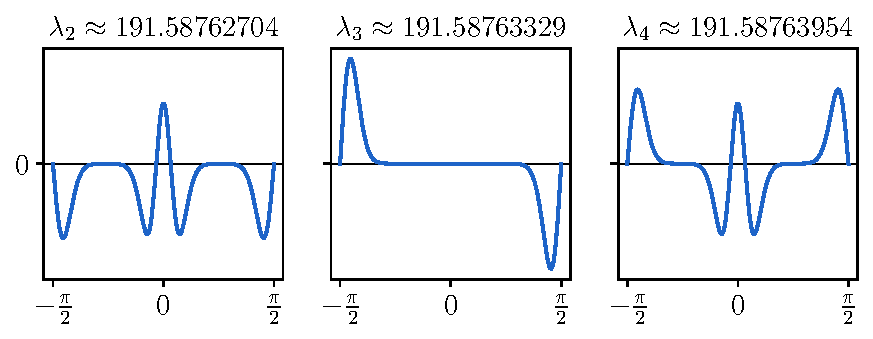
\includegraphics[width=1\textwidth]{img/chapter2/pyslise_test/coffey_evans_eigenfunctions.pdf}
    \end{center}
    \caption{\label{ce_fig}A plot of the eigenfunctions $y_2$, $y_3$ and $y_4$ of the Coffey-Evans problem~(\ref{ce}) with $\beta=25$.}
\end{figure}

The second version of this algorithm is useful in combination with other libraries that expect a function as input (in contrast to a list of function evaluations). For example the \texttt{plot}-function available in Sage:
% \begin{noindent}
\begin{python}
from pyslise import PysliseHalf

# defining the problem, with half range reduction
beta = 25
problem = PysliseHalf(
    lambda x: -2*beta*cos(2*x) + (beta*sin(2*x))^2,
    pi/2, tolerance=1e-8)

# calculating eigenvalues with index 2, 3 and 4
# with boundary conditions (y, y') = (0, 1)
for i, E in problem.eigenvaluesByIndex(2, 5, (0,1)):
    # calculating the corresponding eigenfunction
    f = problem.eigenfunctionCalculator(E, (0, 1))

    # plotting f
    plot(lambda x: f(x)[0], (-pi/2, pi/2)).show()
\end{python}
% \end{noindent}

The result of this code is given in Figure~\ref{ce_fig}.


\subsection{Truncated hydrogen potential}

Lastly we will take a look at the truncated hydrogen potential \cite{pryce_sltstpak_1999}:

\begin{equation}
    V(x) = -\frac{1}{x} + \frac{2}{x^2}  \qquad y(0)=y(1000)=0 \,. \label{thp}
\end{equation}
The lower eigenvalues are a good approximation for the eigenvalues of the non truncated problem ($x \in \left[0, \infty\right[$). For completeness, we also provide a code example to find the first eigenvalues. This is very similar to the previous examples.

% \begin{noindent}
\begin{python}
from pyslise import Pyslise

def V(x):
return -1/x + 2/x**2

hydrogen = Pyslise(V, 0, 1000, tolerance=1e-8)
print(hydrogen.eigenvaluesByIndex(
                    0, 10, (0, 1), (0, 1)))
\end{python}
% \end{noindent}

The potential is unbounded for the left endpoint of the integration interval, thus this is a singular problem. Matslise 2.0 is well-suited for singular problems. It contains a lot of routines and checks to identify and work around singularities of the problem. For efficiency reasons Pyslise is not.

Despite these shortcomings Pyslise is still faster and more accurate. We do note that speedup is less significant than for non-singular problems. In Table~\ref{tab:c2_tab7} we see that Pyslise is at least as accurate as Matslise and approximately 4 times faster (in contrast to 20 times for the Mathieu en Coffey-Evans problems).

\begin{table}
    \begin{center}
        \begin{tabular}[]{rrr}
            \toprule
                               & Matslise 2.0     & Pyslise         \\
            \midrule
                               & $30.96\text{ms}$ & $7.09\text{ms}$ \\
            $-0.0625000000000$ & $2.1$ ($-12$)    & $8.9$ ($-15$)   \\
            $-0.0277777777778$ & $4.9$ ($-12$)    & $-2.2$ ($-15$)  \\
            $-0.0156250000000$ & $3.4$ ($-12$)    & $-9.0$ ($-16$)  \\
            $-0.0100000000000$ & $9.4$ ($-13$)    & $-2.7$ ($-15$)  \\
            $-0.0069444444444$ & $-1.1$ ($-12$)   & $1.2$ ($-13$)   \\
            $-0.0051020408163$ & $-2.3$ ($-12$)   & $-6.3$ ($-13$)  \\
            $-0.0039062500000$ & $-2.9$ ($-12$)   & $-2.3$ ($-13$)  \\
            $-0.0030864197531$ & $-3.0$ ($-12$)   & $1.1$ ($-13$)   \\
            $-0.0025000000000$ & $-2.7$ ($-12$)   & $-9.6$ ($-14$)  \\
            $-0.0020661157025$ & $-1.9$ ($-12$)   & $1.6$ ($-14$)   \\
                               &                  &                 \\
            \bottomrule
        \end{tabular}
        \caption{\label{tab:c2_tab7}The first 10 eigenvalues for the truncated hydrogen problem~(\ref{thp}),
            the execution times and the errors obtained with Matslise 2.0 and Pyslise for a tolerance of $10^{-8}$.  }
    \end{center}
\end{table}

All eigenfunctions are computed in both algorithms with a maximal error of less than $10^{-9}$, with timings similar to the previous test problems.

\section{Implementation challenges}

\todo{Prose}
\todo{UML diagram}

\begin{enumerate}
    \item Template on scalar type.
    \item Unifying different types of solvers. (Normal, HalfRange, SturmLiouville)
    \item Generate formula code
          \begin{enumerate}
              \item Symbolic computation
              \item For systems of equations, non-commutative symbolic computation
              \item Helping the compiler with intermediates
              \item Compiler difficulties
          \end{enumerate}
    \item Memory management:
          \begin{enumerate}
              \item Shared pointers in \cpp{}.
              \item Ownership of sectors.
              \item Eigenfunctions should keep the original problem alive:
                    % \begin{noindent}
\begin{python}
eigenfunctions = []
for q in [1,10,100]:
    mathieu = Pyslise(lambda x: q*x, 0, pi)
    i, E, f = mathieu.eigenpairs(5,6)[0]
    eigenfunctions.append(f)
\end{python}
% \end{noindent}
          \end{enumerate}
    \item Building a Python-package
\end{enumerate}

\stopchapter
